% ---------------------------------------------------------------------------------------------------------------
% TEMPLATE PARA TRABALHO DE CONCLUSÃO DE CURSO
% Esse template foi adaptado para as normas de TCC dos cursos da Unidade Acadêmica de Informação 
% e Comunicação do IFPB a partir do modelo fornecido pela:
%------------------
% Universidade Tecnológica Federal do Paraná - UTFPR
% Customização da classe abnTeX2 (http://www.abntex.net.br/) para as normas da UTFPR
%
% Projeto hospedado em: <link git>
% Autores: Diego Marczal  <>
% 	   Michael Vornes <https://github.com/mvornes>
%
%----------------------------------------------------------------------------------------------------------------
% Codificação: UTF-8
% LaTeX:  abnTeX2          
% ---------------------------------------------------------------------------------------------------------------


% CARREGA CLASSE PERSONALIZADA DO  IFPB--------------------------------------------------------------------
\documentclass[%twoside,                   % Impressão em frente e verso
    	        oneside,                   % Impressão apenas frente
]{configuracoes/ifpb-abntex2}


% INCLUI ARQUIVOS DE CONFIGURAÇÕES-------------------------------------------------------------------------------
% REFERÊNCIAS------------------------------------------------------------------
\usepackage[%
    alf,
    abnt-emphasize=bf,
    bibjustif,
    recuo=0cm,
    abnt-url-package=url,       % Utiliza o pacote url
    abnt-refinfo=yes,           % Utiliza o estilo bibliográfico abnt-refinfo
    abnt-etal-cite=3,
    abnt-etal-list=3,
    abnt-thesis-year=final
]{abntex2cite}                  % Configura as citações bibliográficas conforme a norma ABNT

% PACOTES----------------------------------------------------------------------
\usepackage{pdfpages}                                       % incluir outros arquivos pdf no documento
\usepackage[utf8]{inputenc}                                 % Codificação do documento
\usepackage[T1]{fontenc}                                    % Seleção de código de fonte
\usepackage{booktabs}                                       % Réguas horizontais em tabelas
\usepackage{color, colortbl}                                % Controle das cores
\usepackage{float}                                          % Necessário para tabelas/figuras em ambiente multi-colunas
\usepackage{graphicx}                                       % Inclusão de gráficos e figuras
\usepackage{icomma}                                         % Uso de vírgulas em expressões matemáticas
\usepackage{indentfirst}                                    % Indenta o primeiro parágrafo de cada seção
\usepackage{microtype}                                      % Melhora a justificação do documento
\usepackage{multirow, array}                                % Permite tabelas com múltiplas linhas e colunas
\usepackage{subeqnarray}                                    % Permite subnumeração de equações
\usepackage{lastpage}                                       % Para encontrar última página do documento
\usepackage{verbatim}                                       % Permite apresentar texto tal como escrito no documento, ainda que sejam comandos Latex
\usepackage{amsfonts, amssymb, amsmath}                     % Fontes e símbolos matemáticos
\usepackage[algoruled, portuguese]{algorithm2e}             % Permite escrever algoritmos em português
%\usepackage[scaled]{helvet}                                % Usa a fonte Helvetica
\usepackage{times}                                          % Usa a fonte Times
%\usepackage{palatino}                                      % Usa a fonte Palatino
%\usepackage{lmodern}                                       % Usa a fonte Latin Modern
\usepackage[bottom]{footmisc}                               % Mantém as notas de rodapé sempre na mesma posição
\usepackage{ae, aecompl}                                    % Fontes de alta qualidade
\usepackage{latexsym}                                       % Símbolos matemáticos
\usepackage{lscape}                                         % Permite páginas em modo "paisagem"
%\usepackage{picinpar}                                      % Dispor imagens em parágrafos
%\usepackage{scalefnt}                                      % Permite redimensionar tamanho da fonte
%\usepackage{subfig}                                        % Posicionamento de figuras
%\usepackage{upgreek}                                       % Fonte letras gregas

% Redefine a fonte para uma fonte similar a Arial (fonte Helvetica)
\renewcommand*\familydefault{\sfdefault}

% CONFIGURAÇÕES DE APARÊNCIA DO PDF FINAL--------------------------------------
\makeatletter
\hypersetup{%
    portuguese,
    colorlinks=true,   % true: "links" coloridos; false: "links" em caixas de texto
    linkcolor=blue,    % Define cor dos "links" internos
    citecolor=blue,    % Define cor dos "links" para as referências bibliográficas
    filecolor=blue,    % Define cor dos "links" para arquivos
    urlcolor=blue,     % Define a cor dos "hiperlinks"
    breaklinks=true,
    pdftitle={\@title},
    pdfauthor={\@author},
    pdfkeywords={abnt, latex, abntex, abntex2}
}
\makeatother

% ALTERA O ASPECTO DA COR AZUL--------------------------------------------------
\definecolor{blue}{RGB}{41,5,195}

% REDEFINIÇÃO DE LABELS---------------------------------------------------------
\renewcommand{\algorithmautorefname}{Algoritmo}
\def\equationautorefname~#1\null{Equa\c c\~ao~(#1)\null}

% CRIA ÍNDICE REMISSIVO---------------------------------------------------------
\makeindex

% HIFENIZAÇÃO DE PALAVRAS QUE NÃO ESTÃO NO DICIONÁRIO---------------------------
\hyphenation{%
    qua-dros-cha-ve
    Kat-sa-gge-los
}



% INCLUI ARQUIVOS DO TRABALHO DE CONCLUSÃO DE CURSO (PRÉ-TEXTUAIS, TEXTUAIS, PÓS-TEXTUAIS)-----------------------

% INSERE CAPA E FOLHA DE ROSTO
% CAPA---------------------------------------------------------------------------------------------------

% ORIENTAÇÕES GERAIS-------------------------------------------------------------------------------------
% Caso algum dos campos não se aplique ao seu trabalho, como por exemplo,
% se não houve coorientador, apenas deixe vazio.
% Exemplos: 
% \coorientador{}
% \departamento{}

% DADOS DO TRABALHO--------------------------------------------------------------------------------------
\titulo{Veículos: Sistema de Gestão de Frotas do TRE-PB}
\titleabstract{Title in English}
\autor{José Ricardo Bettini Pacola}
\autorcitacao{PACOLA, José Ricardo Bettini} % Sobrenome em maiúsculo
\local{João Pessoa - PB}
\data{04/2019}

% NATUREZA DO TRABALHO-----------------------------------------------------------------------------------
% Opções: 
% - Trabalho de Conclusão de Curso (se for Graduação)
% - Dissertação (se for Mestrado)
% - Tese (se for Doutorado)
% - Projeto de Qualificação (se for Mestrado ou Doutorado)
\projeto{Relatório de Estágio}

% TÍTULO ACADÊMICO---------------------------------------------------------------------------------------
% Opções:
% - Bacharel ou Tecnólogo (Se a natureza for Trabalho de Conclusão de Curso)
% - Mestre (Se a natureza for Dissertação)
% - Doutor (Se a natureza for Tese)
% - Mestre ou Doutor (Se a natureza for Projeto de Qualificação)
\tituloAcademico{Tecnólogo}

% ÁREA DE CONCENTRAÇÃO E LINHA DE PESQUISA---------------------------------------------------------------
% Se a natureza for Trabalho de Conclusão de Curso, deixe ambos os campos vazios
% Se for programa de Pós-graduação, indique a área de concentração e a linha de pesquisa
\areaconcentracao{}
\linhapesquisa{}

% DADOS DA INSTITUIÇÃO-----------------------------------------------------------------------------------
% Se a natureza for Trabalho de Conclusão de Curso, coloque o nome do curso de graduação em "programa"
% Formato para o logo da Instituição: \logoinstituicao{<escala>}{<caminho/nome do arquivo>}
\instituicao{Instituto Federal de Educação, Ciência e Tecnologia da Paraíba}
\departamento{Unidade Acadêmica de Informação e Comunicação}
\programa{Curso Superior de Tecnologia em Sistemas para Internet}
\logoinstituicao{0.4}{dados/figuras/logo-instituicao2.png} 

% DADOS DOS ORIENTADORES---------------------------------------------------------------------------------
\orientador{Fausto V\'eras Maranh\~ao Ayres}
%\orientador[Orientadora:]{Nome da orientadora}
\instOrientador{Instituto Federal da Para\'iba}

\coorientador{}
%\coorientador[Coorientadora:]{Nome da coorientadora}
\instCoorientador{Instituição do coorientador}

\coordenador{C\^andido Jos\'e Ramos do Egypto}
\supervisor{Francisco Jos\'e Rodrigues Gomes}
\empresa{Tribunal Regional Eleitoral da Para\'{\i}ba}
\dataInicio{10/04/2017}
\dataFim{10/04/2019}
% FOLHA DE ROSTO--------------------------------------------------------------------------------------------------------

% TRABALHO DE CONCLUSÃO DE CURSO/RELATÓRIO DE ESTÁGIO SUPERVISIONADO
 \preambulo{{\imprimirprojeto} Supervisionado apresentado à disciplina Estágio Supervisionado do {\imprimirprograma} do {\imprimirinstituicao}, como requisito parcial para a obtenção do grau de {\imprimirtituloAcademico} em Tecnologia de Sistemas para Internet.}

% DISSERTAÇÃO DE MESTRADO
% \preambulo{{\imprimirprojeto} apresentada ao Programa de \mbox{Pós-graduação} da {\imprimirinstituicao}, como requisito parcial para obtenção do título de {\imprimirtituloAcademico}.}

% TESE DE DOUTORADO
% \preambulo{{\imprimirprojeto} apresentada ao Programa de \mbox{Pós-graduação} da {\imprimirinstituicao}, como requisito parcial para a obtenção do título de {\imprimirtituloAcademico}.}

% PROJETO DE QUALIFICAÇÃO DE MESTRADO OU DOUTORADO
%\preambulo{{\imprimirprojeto} apresentado ao Programa de \mbox{Pós-graduação} da {\imprimirinstituicao}, como requisito parcial para a obtenção do título de {\imprimirtituloAcademico}.}

% OBSERVAÇÕES-----------------------------------------------------------------------------------------------------------
% Altere este arquivo APENAS comentando as linhas que não se aplicam ao tipo de trabalho acadêmico desejado.


% -----------------------------------------------------------------------------
% Folha de Aprovação
% -----------------------------------------------------------------------------

\textopadraofolhadeaprovacao{}

% -----------------------------------------------------------------------------
% Este documento foi mantido apenas para preservar a paginação do trabalho
% acadêmico final, após a inserção da folha de aprovação fornecida
% -----------------------------------------------------------------------------


\begin{document}

\pretextual
\imprimircapa                                               	           % Comando para imprimir Capa
\imprimirfolhaderosto{}                                     		   % Comando para imprimir Folha de rosto
\imprimirfolhadeaprovacao
% INSERE ELEMENTOS PRÉ-TEXTUAIS
% DEDICATÓRIA------------------------------------------------------------------

\renewcommand{\dedicatorianame}{DEDICATÓRIA}

\begin{dedicatoria}

A Deus, a família e aos amigos que são a base e o caminho para um futuro sólido e construtivo. 

\end{dedicatoria}
          			   % Dedicatória
% AGRADECIMENTOS---------------------------------------------------------------

\begin{agradecimentos}[AGRADECIMENTOS]

    Agradeço a Deus e ao meu Anjo da Guarda  por me acompanharem em todos os momentos da minha vida. 
    À família por todo amparo e formação social, neste caso representada pelos meus Pais, meu Irmão, minha Esposa, Enteada e Filho.
    A todos os amigos que fiz ao longo dessa jornada, pois foram com eles que dividi minhas ansiedades e alegrias. 
    A todos os Docentes que dedicam a vida na formação de indivíduos conscientes e responsáveis, em especial aos Docentes do Instituto Federal da Paraíba, pois me surpreenderam desde o primeiro instante com a qualidade e dedicação em que realizam seu trabalho.

    Antes mesmo de sair de Mato Grosso e chegar à Paraíba percebi que seria bem vindo nessa terra. Ainda analisando as possibilidades de vir, entrei em contato com a coordenação do curso de TSI solicitando informações sobre a inscrição do processo seletivo especial, que precisava ser feito pessoalmente. Então a extraordinária e dedicada Prof.ª Valéria, coordenadora ná época, pediu que eu enviasse os documentos junto com uma procuração que ela realizaria a inscrição para mim. Nesse momento vi as portas se abrindo para mim e minha família em uma nova vida que estava por vir. Fica aqui o agradecimento especial a Prof.ª Valéria e ao povo paraibano que nos acolheram.

    Gostaria de dedicar um agradecimento especial a alguns professores que se destacaram pelo amor a profissão e a arte de ensinar. Dentre eles enfatizo a Prof.ª Valéria, que sempre demonstrou muito empenho e paixão ao apresentar a disciplina de algorítimos para os novatos, o Prof.º Fausto que sempre foi um grande amigo, rendendo boas discussões sobre tecnologias e mercado de trabalho, o Prof.º Jaildo pela sua ética impecável, o Prof.º Fred que faz jus ao apelido adquirido ao longo de sua profissão que é ``O Mito" \space lembrado e enfatizado por gerações de turmas do curso de TSI, o Prof.º Dênio pelo domínio impecável de sua disciplina, a Prof.ª Damires por toda sua capacidade, classe e ética impecáveis ao conduzir suas aulas, a Prof.ª Heremita e Prof.ª Nadja pelas calorosas discussões sobre gestão, analise e execução de projetos em suas aulas e também o Prof.º Paulo que apresentou sua disciplina de maneira respeitosa e com muito amor.
    
    Agradeço também a todos os amigos e que fiz durante minha jornada no TRE-PB. Em especial ao Sr. Francisco (Chico) por toda sua atenção e dedicação ao trabalho, sempre pronto a atender e encontrar soluções, ao Rômullo e Leonel pela paciência, capacidade técnica e paixão pela profissão, que sempre estiveram dispostos a me auxiliar em dificuldades técnicas explicando tudo com muita riqueza de detalhes. Agradeço também a todos os amigos estagiários que passaram durante o tempo em que estive, sempre companheiros prontos a aprender e ensinar.

    Para finalizar deixo mais um agradecimento aos meus Pais que sempre acreditaram no caminho da educação e nos resultados que ela traz e também a minha esposa e companheira Walkiria que em todos os momentos esteve ao meu lado me apoiando e acreditando, pois sem eles essa jornada com certeza seria muito mais difícil.

\end{agradecimentos}
        			   % Agradecimentos
% EPÍGRAFE---------------------------------------------------------------------

\renewcommand{\epigraphname}{EPÍGRAFE}

\begin{epigrafe}

\textit{Devemos mudar nossa atitude tradicional em relação à construção de programas. Em vez de imaginar que nossa principal tarefa é instruir o computador sobre o que ele deve fazer, vamos imaginar que nossa principal tarefa é explicar a seres humanos o que queremos que o computador faça. (Donald E. Knuth, Literate Programming).}

\end{epigrafe}

% OBSERVAÇÕES------------------------------------------------------------------
% Altere o texto para inserir a epígrafe do seu trabalho

              			   % Epígrafe
% RESUMO--------------------------------------------------------------------------------

\begin{resumo}[RESUMO]
\begin{SingleSpacing}

% Não altere esta seção do texto--------------------------------------------------------
%\imprimirautorcitacao. \imprimirtitulo. \imprimirdata. \pageref {LastPage} f. \imprimirprojeto\ – \imprimirprograma, \imprimirinstituicao. \imprimirlocal, \imprimirdata.\\
%---------------------------------------------------------------------------------------

% Focar no que foi desenvolvido ....

Nesse relatório de estágio, requisito para conclusão do Curso Superior de Tecnologia em Sistemas para Internet, são apresentadas atividades referentes a aplicação do Modelo de Desenvolvimento de Software no Veículos: Sistema de Gestão de Frotas do TRE-PB. Minha atuação se estendeu por todo o fluxo do modelo de desenvolvimento, participando da análise do problema, ajudando a elicitar histórias de usuários e medir o tamanho das tarefas com a equipe. Implementando classes em Java da camada de modelo com seus respectivos mapeamentos com as tabelas no banco utilizando JPA com Hibernate e o Spring, bem como criando e executando os \textit{scripts} no banco de dados. Implementando classes da camada de controle com suas respectivas regras de negócio e classes da camada de acesso ao banco, realizando operações como um CRUD básico e consultas utilizando JPQL. Na camada de visão utilizamos o JSF com Primefaces para construção do HTML dinâmico juntamente com CSS3 como folhas de estilo e Javascript para execução de lógicas no \textit{browser} do lado do cliente. Esse projeto colaborou profundamente para a fixação dos conhecimentos adquiridos no decorrer do curso, principalmente nas tecnologias: Java, JSF, SQL e SVN. O principal objetivo do estágio foi utilizar, na prática, os conhecimentos obtidos ao longo do curso, bem como aprender conceitos e tecnologias extras, adquirir experiência com a rotina de trabalho e principalmente aprender a codificar em equipe utilizando versionamento de código, seguindo todas as etapas previstas no Modelo de Desenvolvimento de Software denominado MODUS. \\

\textbf{Palavras-chave}: Java. JSF. SQL. Gestão. Desenvolvimento. Equipe.

\end{SingleSpacing}
\end{resumo}

             			   % Resumo em Português
% ABSTRACT--------------------------------------------------------------------------------

\begin{resumo}[ABSTRACT]
\begin{SingleSpacing}

% Não altere esta seção do texto--------------------------------------------------------
\imprimirautorcitacao. \imprimirtitleabstract. \imprimirdata. \pageref {LastPage} f. \imprimirprojeto\ – \imprimirprograma, \imprimirinstituicao. \imprimirlocal, \imprimirdata.\\
%---------------------------------------------------------------------------------------

Elemento obrigatório em tese, dissertação, monografia e TCC. É a versão do resumo em português para o idioma de divulgação internacional. Deve ser antecedido pela referência do estudo. Deve aparecer em folha distinta do resumo em língua portuguesa e seguido das palavras representativas do conteúdo do estudo, isto é, das palavras-chave. Sugere-se a elaboração do resumo (Abstract) e das palavras-chave (Keywords) em inglês; para resumos em outras línguas, que não o inglês, consultar o departamento / curso de origem.\\

\textbf{Keywords}: Java. JEE. JSF, Gerenciamento, Projeto, Veículos.

\end{SingleSpacing}
\end{resumo}

% OBSERVAÇÕES---------------------------------------------------------------------------
% Altere o texto inserindo o Abstract do seu trabalho.
% Escolha de 3 a 5 palavras ou termos que descrevam bem o seu trabalho 
             		           % Resumo em Inglês
% Lista de Figuras----------------------------------------------------------------

\pdfbookmark[0]{\listfigurename}{lof}
\listoffigures*
\cleardoublepage

% OBSERVAÇÕES---------------------------------------------------------------------
% Este arquivo não precisa de ser alterado, pois a lista é gerada automaticamente.
   % Lista de Figuras
%% LISTA DE QUADROS----------------------------------------------------------------

\renewcommand{\listofquadrosname}{LISTA DE QUADROS}

\pdfbookmark[0]{\listofquadrosname}{loq}
\listofquadros*
\cleardoublepage

% OBSERVAÇÕES---------------------------------------------------------------------
% Este arquivo não necessita de ser editado. A lista é gerada automaticamente.
   % Lista de Quadros
%% LISTA DE TABELAS-------------------------------------------------------------

\pdfbookmark[0]{\listtablename}{lot}
\listoftables*
\cleardoublepage

% OBSERVAÇÕES-------------------------------------------------------------------
% Este arquivo não precisa ser alterado, pois a lista é gerada automaticamente.
         		   % Lista de Tabelas
% LISTA DE ABREVIATURAS E SIGLAS----------------------------------------------------------

\begin{siglas}
    \item[ABNT] Associação Brasileira de Normas Técnicas
    \item[DECOM] Departamento de Computação
    \item[PDS] Plano de Desenvolvimento de Software
    \item[MODUS] Modelo de Desenvolvimento de Software
    \item[SEDES] Seção de Desenvolvimento de Sistemas
    \item[SISBAN]Seção de Impantação de Sistemas e Banco de dados
    \item[TRE-PB] Tribunal Regional Eleitoral da Paraíba
    \item[IFPB] Instituto Federal de Educação da Paraíba
    \item[SQL] Structured Query Language
    \item[DBA] DataBase Administrator
    \item[JSF] JavaServer Faces
    \item[SVN] Apache Subversion
\end{siglas}

% OBSERVAÇÕES-----------------------------------------------------------------------------
% Altere a lista acima para definir os acrônimos e siglas utilizados neste trabalho
          		   % Lista de Abreviaturas e Siglas
%% LISTA DE SÍMBOLOS------------------------------------------------------------

\begin{simbolos}
    \item[$ \Gamma $] Letra grega Gama
    \item[$ \lambda $] Comprimento de onda
    \item[$ \in $] Pertence
\end{simbolos}

% OBSERVAÇÕES-------------------------------------------------------------------
% Altere a lista acima para definir os símbolos utilizados no trabalho
        		   % Lista de Símbolos
%% LISTA DE ALGORITMOS----------------------------------------------------------

\newcommand{\algoritmoname}{Algoritmo}
\renewcommand{\listalgorithmcfname}{LISTA DE ALGORITMOS}

\floatname{algocf}{\algoritmoname}
\newlistof{listofalgoritmos}{loa}{\listalgoritmoname}
\newlistentry{algocf}{loa}{0}

\counterwithout{algocf}{chapter}
\renewcommand{\cftalgocfname}{\algoritmoname\space}
\renewcommand*{\cftalgocfaftersnum}{\hfill--\hfill}

\pdfbookmark[0]{\listalgorithmcfname}{loa}
\listofalgorithms
\cleardoublepage

% OBSERVAÇÕES------------------------------------------------------------------
% Este arquivo não precisa ser alterado, pois a lista é gerada automaticamente.
   % Lista de Algoritmos
% SUMÁRIO----------------------------------------------------------------------

\renewcommand{\contentsname}{SUMÁRIO}

\pdfbookmark[0]{\contentsname}{toc}
\tableofcontents*
\cleardoublepage

% OBSERVAÇÕES-------------------------------------------------------------------
% Este arquivo não precisa ser alterado, pois o sumário é gerado automaticamente.
               			   % Sumário

\textual
% INSERE ELEMENTOS TEXTUAIS
% INTRODUÇÃO-------------------------------------------------------------------

\chapter{Introdução}
\label{chap:introducao}

Este relatório descreve as atividades realizadas, no que diz respeito ao planejamento, desenvolvimento e execução de um dos projetos desenvolvidos pela SEDES, denominado de Veículos – Sistema de gestão de frotas do TRE-PB. O mesmo foi executado no exercício do estágio supervisionado no Tribunal Regional Eleitoral da Paraíba, localizado no Centro em João Pessoa.

O projeto teve inicio em abril de 2017 e a versão 1.0 foi entregue na metade de maio de 2017 e continha cadastros inciais como colaboradores e veículos. A versão 1.1 se estendeu até julho de 2017 e continha as principais funcionalidades da aplicação que de fato iriam realizar o controle das viagens. O projeto tinha previsão para ser concluído em até dois meses, porém uma mudança substancial do modelo teve que ser efetuada durante a fase de desenvolvimento da versão 1.1, como pode ser visto na ata de reunião descrita na \autoref{fig:figura-ata1} e então o projeto se estendeu para cinco meses. Ele foi supervisionado pelo chefe da SEDES, Francisco Gomes, bem como acompanhado pelo supervisor técnico, que é o desenvolvedor responsável pelo projeto que também precisou ser substituído, todos efetivos no quadro do Tribunal. A equipe no projeto ficou composta por 1 gerente e 3 desenvolvedores, sendo 1 supervisor técnico e 2 estagiários, 1 Product Owner e 1 DBA responsável pelo gerenciamento do banco de dados, este lotado na SISBAN.

O sistema passou a ser utilizado em sua plenitude a partir de agosto de 2017 e em 2018 terminou o ano sendo o 4º sistema mais usado em todo o TRE com 23.375 transações conforme \autoref{fig:figura-ranking2018}. Já em 2019, até março foram registradas 4.006 transações já sendo o 3º sistema mais utilizado como pode ser visto na \autoref{fig:figura-ranking2019}.

\begin{figure}[!htb]
    \centering
    \caption{Veículos - Ranking 2018}
    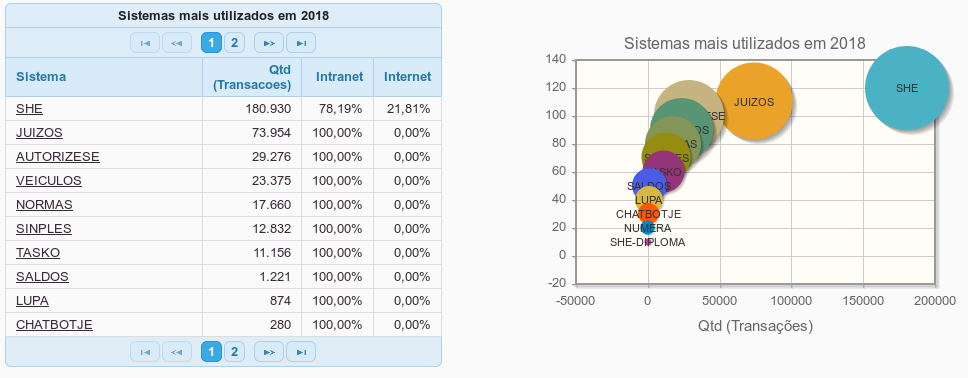
\includegraphics[width=0.75\textwidth]{./dados/figuras/ranking2018.png}
    \fonte{SEDES}
    \label{fig:figura-ranking2018}
\end{figure}

\begin{figure}[!htb]
    \centering
    \caption{Veículos - Ranking 2019}
    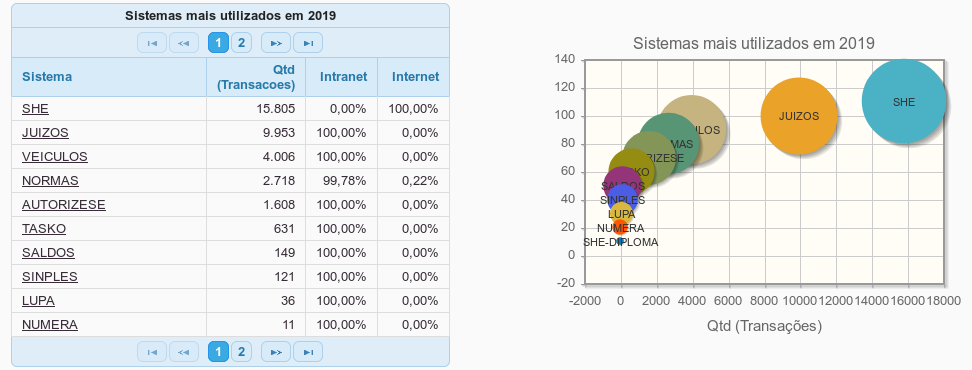
\includegraphics[width=0.75\textwidth]{./dados/figuras/ranking2019.png}
    \fonte{SEDES}
    \label{fig:figura-ranking2019}
\end{figure}

Nesse relatório serão explanados, tanto os conhecimentos teóricos, quanto os práticos, descrevendo todas as etapas do projeto. Também estarão presentes neste relatório informações referentes à empresa e sobre a unidade da empresa onde o projeto foi executado, além de informações sobre infra-estrutura.
Por fim, serão mencionadas as correlações entre o conteúdo visto em sala de aula e o que foi feito na prática, bem como as principais dificuldades encontradas durante a execução do projeto.


\section{Objetivo}
\label{sec:objetivo}

\subsection{Objetivo geral}
\label{sec:objetivoGeral}
Auxiliar no desenvolvimento dos ativos, soluções web desenvolvidas pela SEDES, participando de todas as atividades contempladas pelas etapas descritas no Modelo de Desenvolvimento de Software adotado pelo TRE-PB.  Para vistas deste relatório será utilizado como referência o projeto \imprimirtitulo. O sistema deve ser capaz de receber solicitações dos usuários e exibi-las em um painel onde o gestor deverá analisar os pedidos e montar as viagens adequando: rotas, disponibilidades dos motoristas e passageiros.

\subsection{Objetivos específicos}
\label{sec:objetivosEspecificos}
Contribuir na implementação do Sistema de Gestão de Frotas, quando possível oferecendo alternativas para a implementação mediante aos conhecimentos adquiridos na graduação. Ganhar experiência com o fluxo de trabalho da uma equipe de desenvolvimento incorporando conceitos de metodologias ágeis e versionamento de código, sendo capaz de resolver conflitos de códigos, quando houver, e evita-los. Trabalhar com reuniões diárias, planejar soluções com a modelagem do negócio especificando suas respectivas histórias de usuários, codificar utilizando as tecnologias e padrões adotados pela equipe, realizar entregas frequentes sempre buscando feedback das releases pelo cliente e gerar documentação explicando as funcionalidades e como utiliza-las. 

% utilizar met. ágeis, trabalhar em equipe, participar de reuniões, documentar, especificar, implementar...

\section{A Empresa}\footnote{http://www.tre-pb.jus.br/institucional/conheca-o-tre-pb/conheca-o-tre-pb}
\label{sec:empresa}
A Justiça Eleitoral é o ramo especializado do Poder Judiciário que visa garantir a lisura, a eficiência e a eficácia do processo eleitoral, contribuindo para o fortalecimento da democracia e a consolidação do Estado de Direito. Compete à Justiça Eleitoral preparar, realizar e apurar as eleições, além de administrar o Cadastro Nacional de Eleitores.
O principal objetivo da Justiça Eleitoral é o gerenciamento do processo eleitoral, através de diretrizes claras e firmes, evitando vícios, abusos e fraudes.
O Tribunal Regional Eleitoral da Paraíba - TRE-PB, órgão máximo da Justiça Eleitoral no Estado, tem como instância superior, em matéria eleitoral, o Tribunal Superior Eleitoral, sediado em Brasília - Distrito Federal. A finalidade do TRE-PB é planejar e coordenar o processo eleitoral nas eleições federais, estaduais e municipais, no âmbito do Estado da Paraíba.
Compete, também, ao Tribunal, julgar os recursos interpostos das decisões dos Juízes e Juntas Eleitorais do Estado, bem como, os processos originários e administrativos do próprio Tribunal; registrar os partidos e candidatos a cargos eletivos de Governador, Senador, Deputado Federal e Estadual, assim como, receber e analisar a prestação de contas dos mesmos, prestadas ao final de cada campanha estadual; analisar as prestações de contas anuais dos órgãos regionais dos partidos políticos; elaborar e fiscalizar o calendário estadual de propaganda eleitoral; proceder à anotação e cancelamento dos diretórios estaduais e municipais dos partidos políticos; julgar as impugnações relativas aos pedidos de registros de candidaturas e as arguições de inelegibilidade; designar os Juízes Titulares das Zonas Eleitorais do Estado da Paraíba e administrar o Cadastro de Eleitores.

\section{Descrição geral das atividades}
\label{sec:descricaoGeralAtividades}
Durante o processo foram utilizadas as metodologias Scrum para gestão e planejamento dos projetos e o Kanban para o controle de fluxo do desenvolvimento. As atividades desenvolvidas no período do estágio foram as seguintes de acordo com as fases: 
\begin{enumerate}
    \item Imersão:
    \begin{enumerate}
        \item Elicitação das histórias de usuário.
        \item Definição do escopo do produto.
        \item Criar estrutura do projeto.
        \item Modelagem de dados.
    \end{enumerate}
   \item Construção:
   \begin{enumerate}
        \item Refinar histórias de usuário.
        \item Estimar histórias.
        \item Codificação de funcionalidades.
        \item Preparar versão para homologação.
        \item Codificar ajustes.
        \item Gerar documentação.
        \item Implantar versão.
   \end{enumerate}
\end{enumerate}

\section{Organização do relatório}
\label{sec:organizacaoRelatorio}
Além desse capítulo, o relatório está dividido em outros três capítulos brevemente descritos abaixo:

\autoref{chap:embasamentoTeorico} - Embasamento Teórico: aborda as tecnologias e linguagens que foram utilizadas durante o estágio, bem como as definições necessárias para a compreensão do processo.

\autoref{chap:atividadesRealizadas} - Atividades Realizadas: apresenta o projeto, no qual as atividades do estagiário foram realizadas, descrevendo os principais conceitos e funcionalidades. Relata as atividades realizadas ao longo do período de estágio descrevendo o fluxo e o processo de desenvolvimento e detalha a implementação de algumas funcionalidades.

\autoref{chap:consideracoesFinais} – Considerações Finais: Apresenta um relato sobre as experiências adquiridas, metas e objetivos alcançados. O quão grande foi a contribuição do estágio na minha formação profissional.
                		            % Introdução
% REVISÃO DE LITERATURA--------------------------------------------------------

\chapter{Embasamento teórico }
\label{chap:embasamentoTeorico}

Este capítulo apresenta uma breve fundamentação dos assuntos e conceitos necessários para a melhor compreensão deste trabalho, dando ênfase aos pontos mais relevantes para a compreensão das atividades realizadas.

A SEDES é uma seção responsável por implementar e realizar manutenções em ativos de TI do TRE-PB. Dessa forma ela se comporta como uma fábrica de \textit{software}, seguindo rigorosos critérios no desenvolvimento de seus produtos, todos documentados em um modelo de desenvolvimento, visando a qualidade e segurança de seus produtos. Técnicas e tecnologias reconhecidas do mercado são utilizadas, dentre elas o algumas metodologias ágeis como SCRUM e KAMBAM, JAVA, ORACLE SQL.

\section{SCRUM}
\label{sec:embasamentoTeoricoSCRUM}

SCRUM é uma metodologia (ou processo) de desenvolvimento iterativo e incremental, utilizada também no gerenciamento e desenvolvimento de \textit{software} de forma ágil.

\begin{citacao}
    O SCRUM assume-se como uma metodologia extremamente ágil e flexível, que tem por objetivo definir um processo de desenvolvimento iterativo e incremental podendo ser aplicado a qualquer produto ou no gerenciamento de qualquer atividade complexa. \cite{Bissi2007}.
\end{citacao}

No SCRUM, os projetos são divididos em Sprints, que são ciclos, geralmente mensais, que representam o tempo no qual um determinado conjunto de atividades deve ser executado. Cada atividade ou funcionalidade a ser implementada no projeto são mantidas em uma lista, chamada de \textit{Product Backlog}. Ao iniciar cada sprint é realizada uma reunião de planejamento, conhecida como \textit{Sprint Planning Meeting}. Nessa reunião, o \textit{Product Owner}, que é a pessoa que define o que está no \textit{Product Backlog}, irá determinar as prioridades e a equipe irá discutir quais atividades ela será capaz de executar naquela sprint. A partir daí, a cada dia dessa sprint é feita uma reunião diária, geralmente realizada no início do dia, denominada de \textit{Daily Scrum}.  Nessa reunião, cada membro da equipe informa o que fez no dia anterior, e são identificados impedimentos e são estabelecidas novas prioridades para o dia atual.

Ao término de uma sprint, a equipe apresenta o que foi implementado, em uma pequena reunião, chamada Sprint Review Meeting. Logo após, é feito um novo planejamento para a próxima Sprint, reiniciando o ciclo, conforme é ilustrado na \autoref{fig:figura-cicloSCRUM}.


\begin{figure}[!htb]
    \centering
    \caption{Exemplo do cliclo SCRUM}
    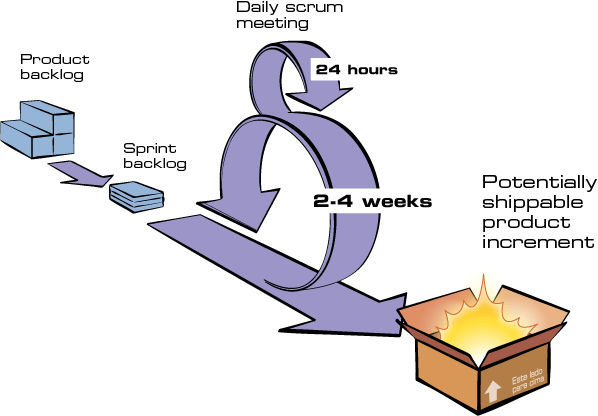
\includegraphics[width=0.7\textwidth]{./dados/figuras/cicloSCRUM}
    \fonte{Site Mindmaster}
    \label{fig:figura-cicloSCRUM}
\end{figure}

Outro conceito do SCRUM é o \textit{Planning Poker}, que é uma técnica utilizada para estimar o prazo de um projeto. Resumidamente, nessa técnica, é usado um conjunto de cartas. Cada carta contém um número que representa pontos. Os números vão de 1 a 100, seguindo a sequência 0, 1, 2, 3, 5, 8, 13, 20, 40, 100. Cada membro da equipe recebe o conjunto de cartas. Escolhido um \textit{ticket} (tarefa), os usuários ao mesmo tempo lançam à mesa a carta com a quantidade de pontos que consideram que vale aquele \textit{ticket} (geralmente, e esse foi o nosso caso, a quantidade de pontos remetia à quantidade de horas que levaríamos para executar aquela tarefa). O processo é repetido para todos os \textit{tickets}. A ideia é instigar a discussão, pois, dificilmente, todos os membros da equipe irão jogar a mesma carta. Somente após um consenso é que o valor final é atribuído à tarefa \cite{Sabbagh2014}.

\section{Java}
\label{sec:embasamentoTeoricoJava}

Java\footnote{http://www.oracle.com/technetwork/pt/java/index.html} é uma linguagem de programação orientada a objetos, lançada em 1995, pela empresa Sun Microsystems, mas que, atualmente, pertence a Oracle \cite{Deitel2009}. A linguagem Java permite o desenvolvimento de \textit{software} para as plataformas \textit{desktop (Standard Edition), mobile (Micro Edition) e \textit{web} (Enterprise Edition)}. O código em Java não é compilado para código nativo, mas sim para um bytecode, que é executado por uma máquina virtual, a JVM (\textit{Java Virtual Machine}). 
O Java é amplamente utilizado ao redor do mundo, principalmente em ambientes coorporativos. No Brasil, o Java é uma das principais linguagens de programação, sendo base para o ensino da Programação Orientada à Objeto na grande maioria dos cursos de programação. Além de ser bastante utilizada em organizações públicas. Isso se deve justamente pelo fato de que o foco do Java é em aplicações de médio a grande porte. Se forem bem usadas as recomendações e práticas do paradigma orientado à objeto, torna-se fácil a manutenção de uma aplicação Java, mesmo sendo de grande porte. Outra característica, que faz do Java uma ótima opção para esse escopo, é o suporte dela as diversas bibliotecas (ou APIs) para os mais diversos trabalhos como relatórios, persistência, gráficos, entre outras. 

\section{JSF}
\label{sec:embasamentoTeoricoJSF}

De acordo com \citeonline{Cordeiro2014}, \textit{desktop (JavaServer Faces)}\footnote{https://javaee.github.io/javaserverfaces-spec/}, ou, mais comumente, JSF, é um \textit{desktop (framework)} MVC para desenvolvimento \textit{web} com Java, que veio para facilitar a construção de \textit{desktop (interfaces)} de usuário. A sua \textit{desktop (interface)} de usuário é baseada em componentes e orientada a eventos, sendo assim, os detalhes de manipulação dos eventos e a organização dos componentes são abstraídas. Com isso, o programador pode se concentrar bem mais na lógica do negócio. O JSF usa como sistema de \textit{template} padrão o \textit{Facelets}.

O JSF estabelece um conjunto de componentes pré-definidos para o desenvolvimento da \textit{desktop (interface)} de usuário. Para acessar esses componentes, ele fornece \textit{tags} JSP. Outra característica interessante é que o JSF permite a reutilização dos componentes em uma página, aumentando a performance de carregamento da mesma. O JSF também faz uso do AJAX em alguns componentes, fazendo com que os processos sejam mais rápidos.

\section{PrimeFaces}
\label{sec:embasamentoTeoricoPrimeFaces}

PrimeFaces\footnote{https://primefaces.org/} é uma biblioteca \textit{Open Source} de componentes para o JSF. Essa biblioteca contribui para que o \textit{software} tenha, o que chamamos de \textit{desktop (interface)} rica, devido ao grande conjunto de componentes. O PrimeFaces utiliza o jQuery2 e jQuery UI. Assim como outros \textit{desktop (frameworks)} para a parte visual do sistema, ele também se preocupa com a responsividade do \textit{layout}.
Os componentes do PrimeFaces foram construídos para usar AJAX por padrão, com isso o desenvolvedor não precisa ter a preocupação de realizar chamadas assíncronas para o servidor. O PrimeFaces também conta com um conjunto de temas (skins), que permite, de forma fácil mudar a aparência das aplicações.
A grande característica do PrimeFaces é a sua simplicidade. Não é necessário configurar nenhum XML. Para utilizá-lo, basta colocar a biblioteca no projeto. Tudo isso está muito bem documentado no site do PrimeFaces, que também possui vários exemplos de código \cite{Civici2015}.

\section{JPA e Hibernate}
\label{sec:embasamentoTeoricoJPA}

Java Persistense API\footnote{ http://www.oracle.com/technetwork/java/javaee/tech/persistence-jsp-140049.html} ou JPA é uma especificação criada em 2006 a partir do Hibernate\footnote{http://hibernate.org/}, que é um \textit{desktop (framework)} de mapeamento objeto-relacional (ORM), tendo em vista que outros \textit{desktop (framework)} estavam surgindo foi necessário criar um padrão com o intuito de resolver o famoso vendor lock-in, ou seja, uma vez usando determinada distribuição, ficava-se preso à mesma \cite[p.~12]{Cordeiro2014}.

A abstração do JPA é a sua maior característica, permitindo que o programador troque o banco de dados sem maiores dificuldades. No projeto Veículos, foi usado o Hibernate através da especificação JPA.O uso da JPA é feito através de anotações na classe que representa o objeto que será persistido. Esse processo de anotar/configurar classes chama-se mapeamento. As classes depois de mapeadas são reconhecidas pelo Hibernate, que faz o seu processo natural de converter esse objeto para uma tabela no banco de dados \cite{Cordeiro2014}.


\section{Spring \textit{desktop (framework)}}
\label{sec:embasamentoTeoricoSpring}

O Spring surgiu em 2003 como uma resposta à complexidade das primeiras especificações do J2EE. Enquanto alguns consideram que Java EE e Spring estão competindo, o Spring é, de fato, complementar ao Java EE. O modelo de programação Spring não abrange a especificação da plataforma Java EE; em vez disso, integra-se com especificações individuais cuidadosamente selecionadas do JavaEE:

\begin{itemize}
    \item \textit{Servlet} API (JSR 340)
    \item \textit{WebSocket} API (JSR 356)
    \item \textit{Concurrency Utilities} (JSR 236)
    \item JSON \textit{Binding} API (JSR 367)
    \item Bean \textit{Validation} (JSR 303)
    \item JPA (JSR 338)
    \item JMS (JSR 914)
\end{itemize}

O \textit{desktop (framework)} também suporta injeção de dependências (JSR 330)  e anotações comuns (JSR 250), que os desenvolvedores de aplicativos podem usar em vez dos mecanismos específicos do Spring.

\subsection{Anotações de Estereótipo}
São anotações usadas para declarar a função que o componente desempenha na aplicação. Por exemplo, a anotação @Repository no Spring \textit{desktop (framework)} é uma marcação para qualquer classe que atenda a função de um repositório (também conhecido como \textit{Data Access Object} ou DAO).

\section{JasperReports}
\label{sec:embasamentoTeoricoJasper}

O JasperReports é um \textit{desktop (framework)} \textit{open source} inteiramente escrito em Java. Ele é um dos mecanismos mais populares para a geração de relatórios na plataforma Java.
O JasperReports nos fornece funcionalidades que permitem criar relatórios complexos de forma estruturada, a partir da elaboração de um \textit{template} \cite{Devmedia2012}.

O \textit{template} é um arquivo XML com a extensão .jrxml. É neste arquivo que é especificada a estrutura do relatório, ou seja, é nele onde informamos os dados que irão compor o relatório, em que posição e de que forma serão exibidos, formando assim um \textit{layout}. Utiliza-se o IReports para diagramação dos elementos de maneira gráfica.

A partir da definição do \textit{template} e com o auxílio do \textit{desktop (framework)} JasperReports é possível gerar relatórios e exportá-los para diversos formatos, como: HTML, PDF e DOC.

\section{Tomcat}
\label{sec:embasamentoTeoricoTomcat}

O Apache Tomcat® é uma implementação open source das tecnologias Java \textit{Servlet}, JavaServer \textit{Pages}, Java \textit{Expression Language} e Java \textit{WebSocket} technologies.

Ele atende parte da especificação JEE com as tecnologias \textit{Servlet} e JSP  e tem a capacidade de atuar também como servidor \textit{web} HTTP escrito puramente em Java. Ele inclui ferramentas para configuração e gerenciamento, o que também pode ser feito editando-se manualmente arquivos de configuração formatados em XML \cite{WikipediaTomcat2018}.

Atualmente o Tomcat está na versão 9.x. Para o projeto foi utilizado o Tomcat 8.0.x tanto nas máquinas de desenvolvimento quanto nos servidores. O TRE-PB faz o uso de múltiplos servidores de produção e homologação com o Tomcat, dividindo assim a carga das aplicações. 

        % Embasamento teórico
% ATIVIDADES REALIZADAS------------------------------------------------------------------

\chapter{Atividades realizadas}
\label{chap:atividadesRealizadas}

Nesse capítulo será explanada minha participação no processo de desenvolvimento do projeto o qual tive a oportunidade de participar desde a concepção, homologação, correção de problemas, criação de uma nova versão com expressiva mudança no modelo de dados e implementação da aplicação em produção.

\section{\imprimirtitulo}
\label{sec:atividadesRealizadasVeiculos}

O projeto \imprimirtitulo \space foi concebido com o objetivo de controlar as solicitações de veículos e as viagens realizadas, promovendo uma melhor gestão da frota de veículos do TRE-PB bem como possibilitando a realização de auditorias com base nos dados contidos no sistema.
O sistema é hoje um ativo de TI que foi desenvolvido pela SEDES e está descrito no catálogo técnico de sistemas da COSIS conforme \autoref{fig:figura-ativoTI}. 

\begin{figure}[!htb]
    \centering
    \caption{Catálogo técnico de sistemas - Veículos}
    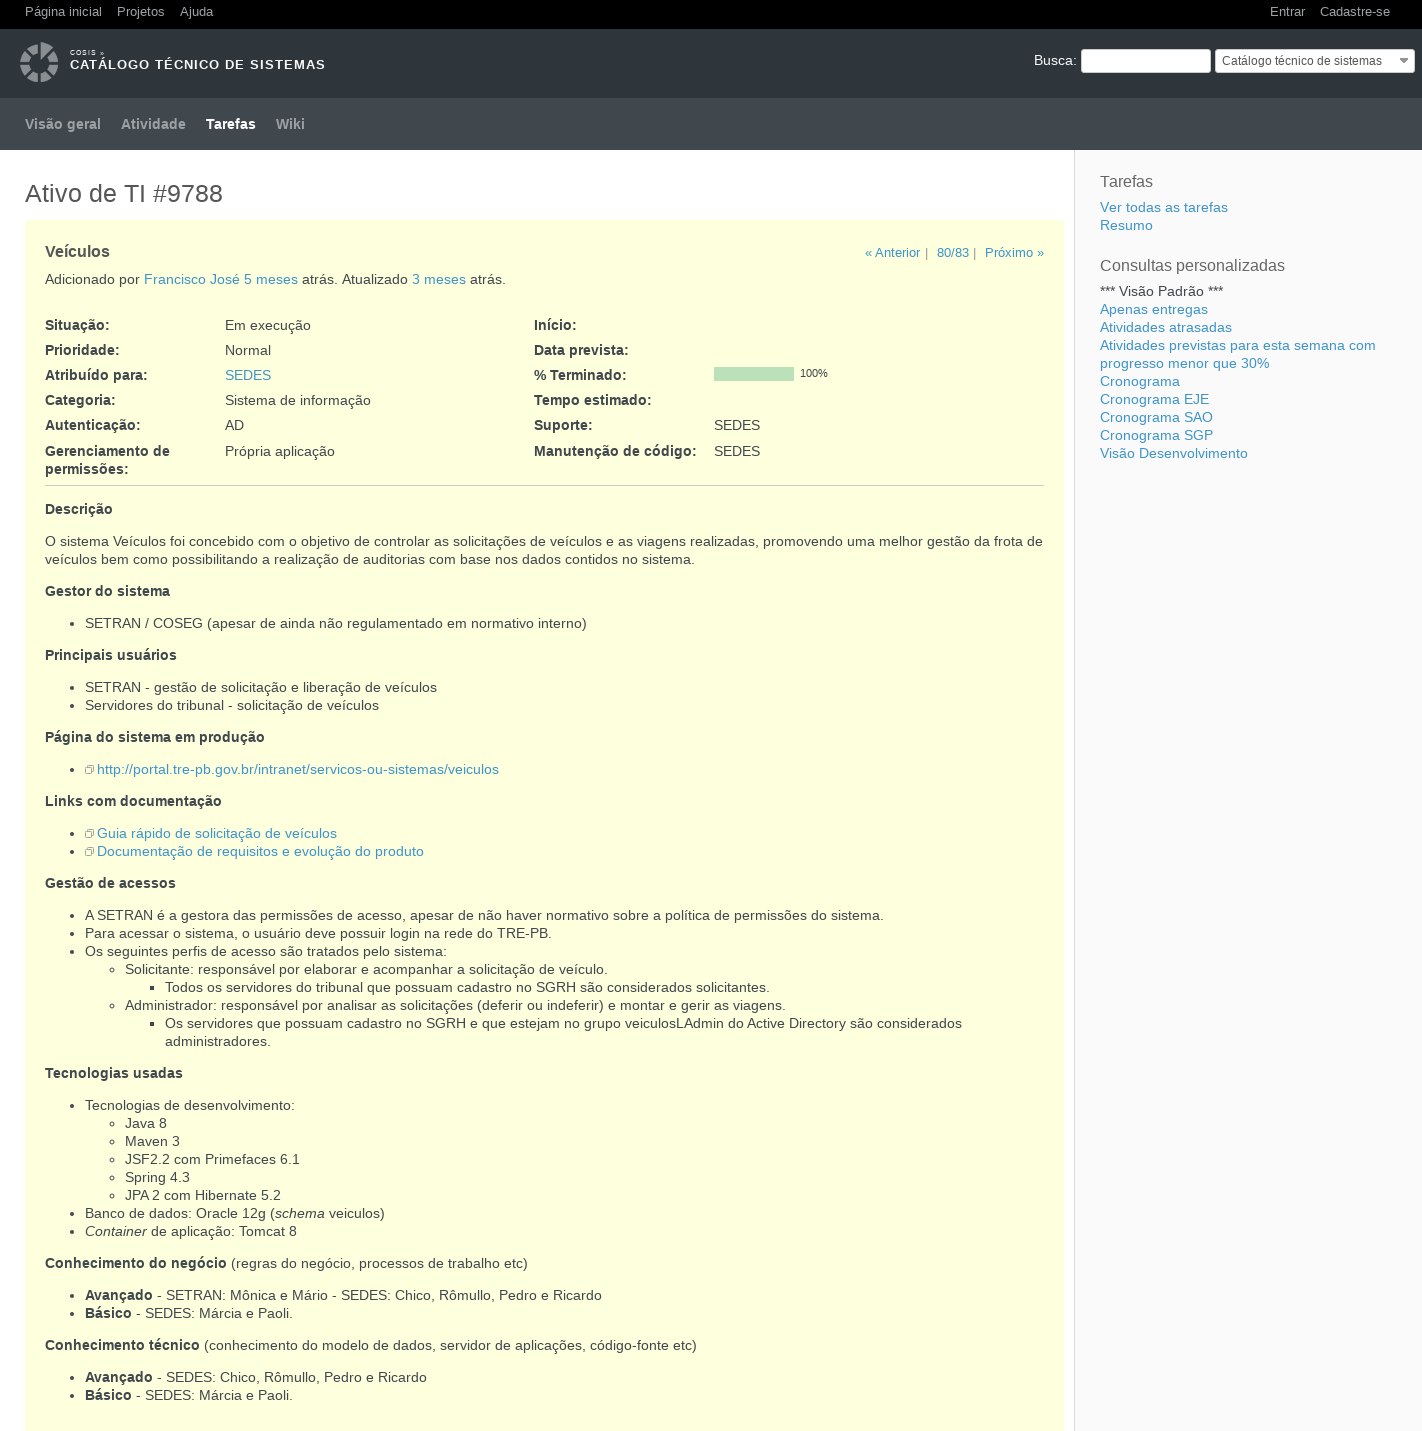
\includegraphics[width=0.75\textwidth]{./dados/figuras/veiculos-ativoTI}
    \fonte{COSIS}
    \label{fig:figura-ativoTI}
\end{figure}

O sistema permite a qualquer membro e servidor lotado no TRE-PB, através do seu login de usuário, solicitar um veículo descrevendo a data, local/trecho, hora de partida, hora de retorno e a atividade que deverá ser realizada como pode ser visto na \autoref{fig:figura-solicitacao}.

\begin{figure}[!htb]
    \centering
    \caption{Veículos - Tela de solicitação}
    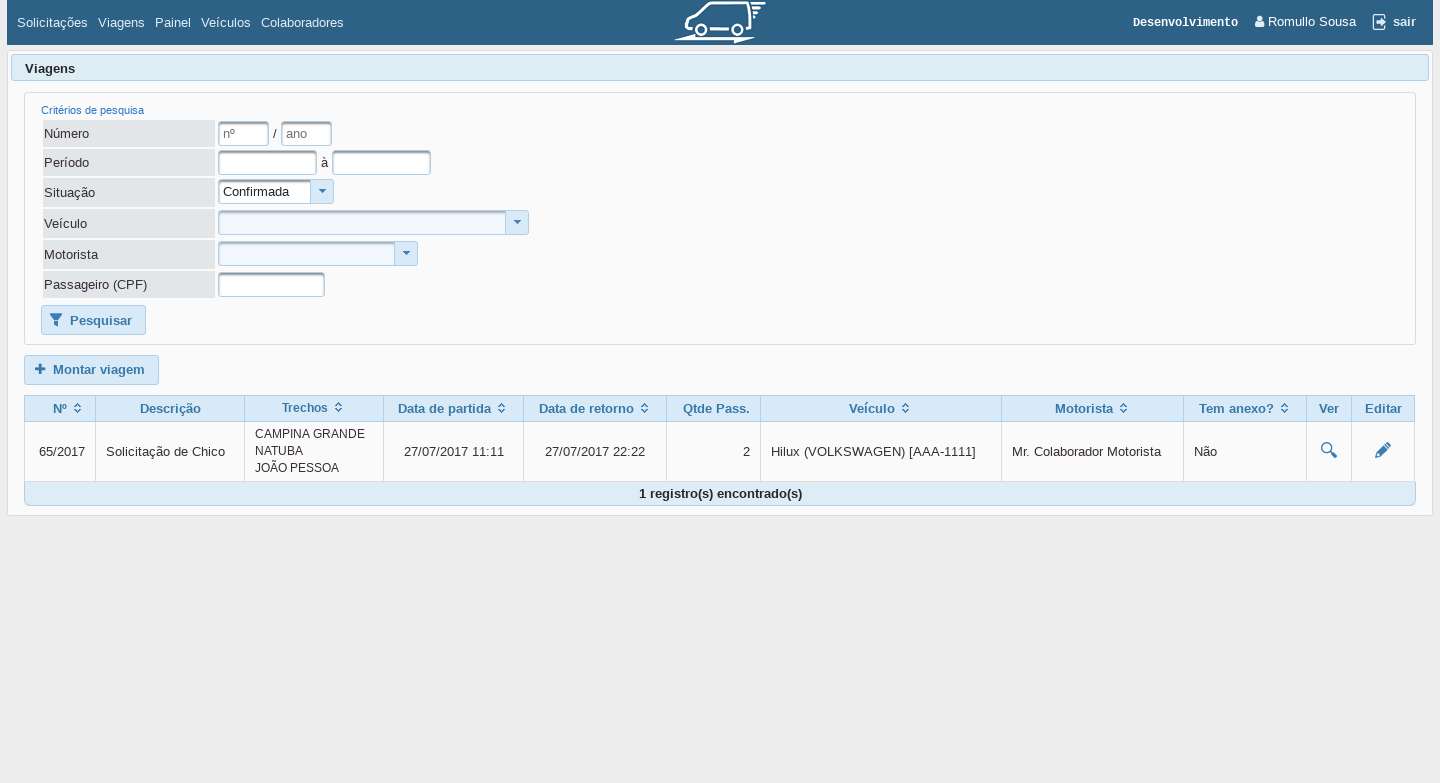
\includegraphics[width=0.75\textwidth]{./dados/figuras/veiculos-tela1.png}
    \fonte{SEDES}
    \label{fig:figura-solicitacao}
\end{figure}

O gestor lotado na COSEG, possui um perfil de administrador e em sua tela recebe as solicitações de todos os servidores e membros. Com a visão de todas as solicitações o gestor tem a possibilidade de analisar passageiros que irão para os mesmos destinos, ou até mesmo na rota, com horários similares e montar as viagens adequando a disponibilidade de motoristas e veículos. Através de um quadro, exibido na figura \autoref{fig:figura-motoristas}, o gestor consegue visualizar a ocupação dos veículos e motoristas pelo horário e dia da semana. Com a viagem montada e deferida pelo gestor, o solicitante recebe uma confirmação em seu e-mail informando os detalhes da viagem. Os motoristas recebem uma guia contendo a autorização e detalhes da viagem como a rota e os passageiros. Nessa guia o motorista deve anotar a quilometragem do veículo e exibir para o vigia que deve conferir os valores e permitir a saída do veículo. No retorno o motorista novamente anota na guia a quilometragem de chegada que é conferida pelo vigia.

A modelagem inicial do sistema, na versão 1.0.0, não possuia uma separação dos modelos entre solicitação e viagem. Isso acabou ocasionando um gargalo no desenvolvimento, pois surgiram feedbacks ao longo das etapas, como pode ser visto na ata de reunião na \autoref{fig:figura-ata1}, em que há casos de uma solicitação necessitar de mais de uma viagem para ser concluída e uma viagem poder atender mais de uma solicitação. A aplicação precisou ser refatorada e um novo prazo foi apresentado.

\begin{figure}[!htb]
    \centering
    \caption{Veículos - Tela de solicitação}
    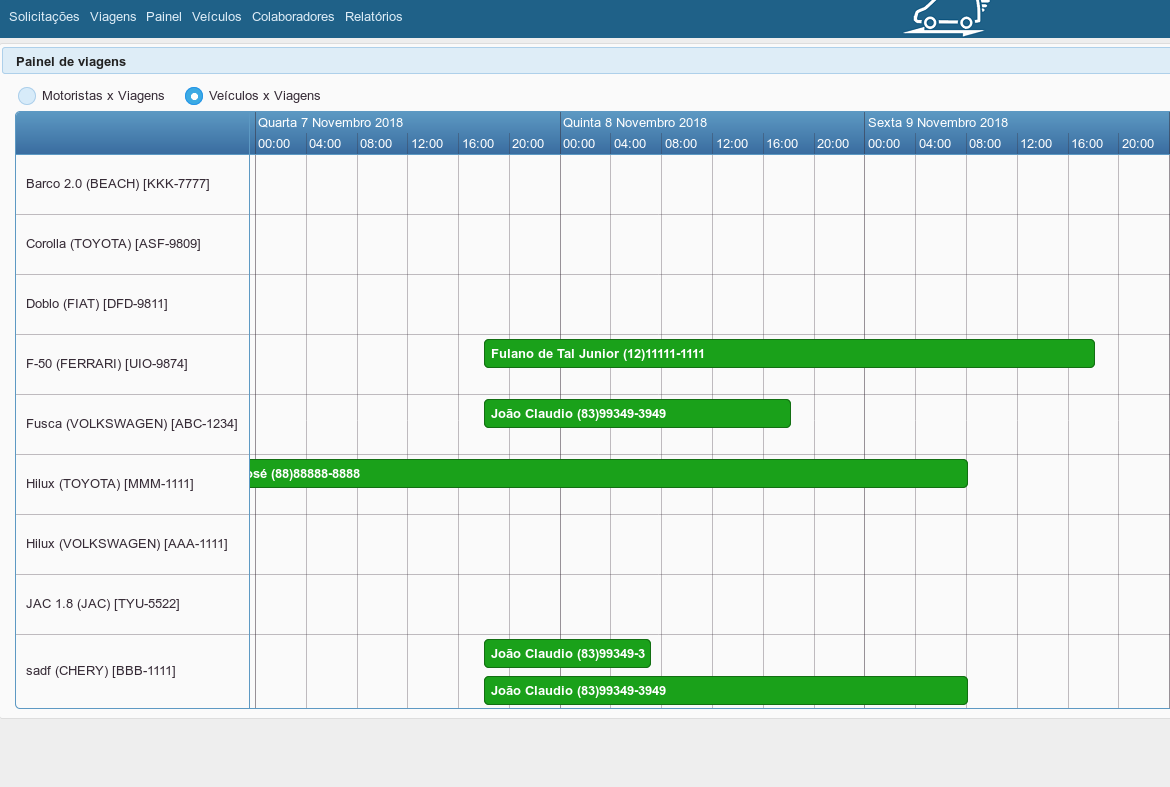
\includegraphics[width=0.75\textwidth]{./dados/figuras/veiculos-tela2.png}
    \fonte{SEDES}
    \label{fig:figura-motoristas}
\end{figure}

\begin{figure}[!htb]
    \centering
    \caption{Ata de reunião - feedback}
    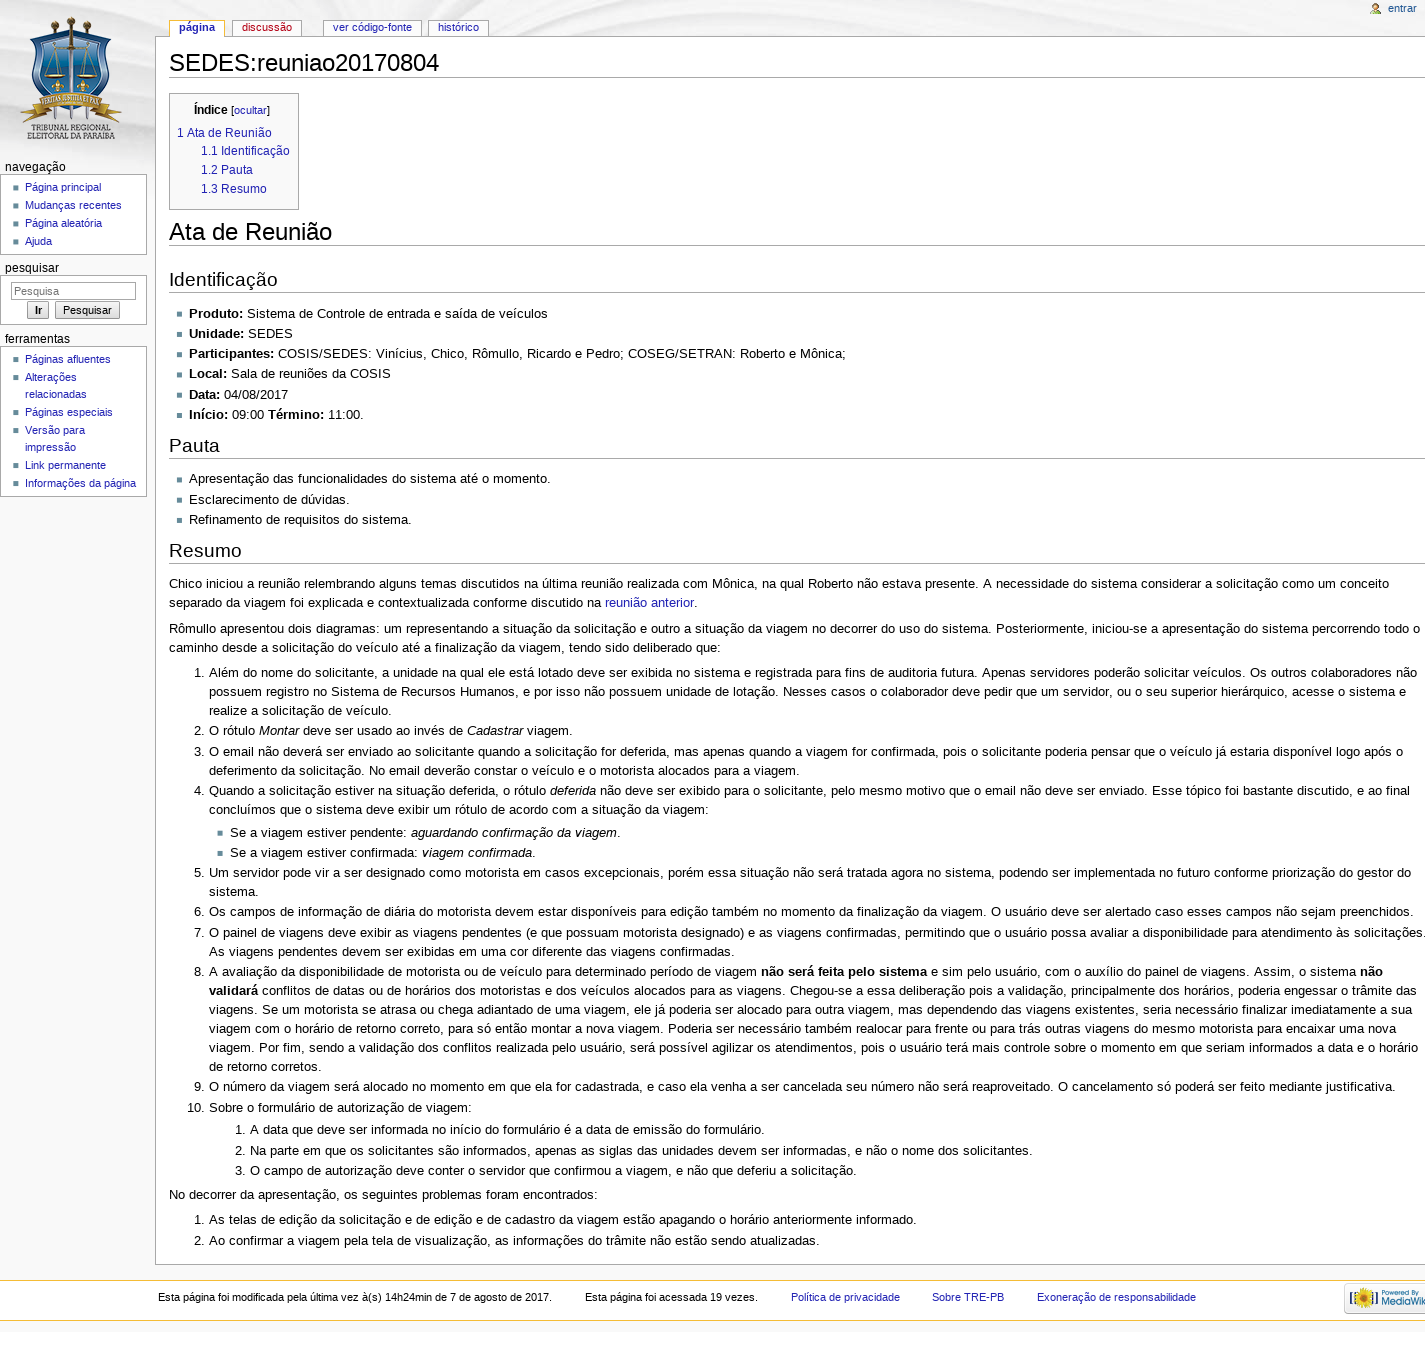
\includegraphics[width=1\textwidth]{./dados/figuras/veiculos-ata1.png}
    \fonte{SEDES}
    \label{fig:figura-ata1}
\end{figure}

O desenvolvimento do sistema passou por todas as etapas de um projeto de software conforme descrição no modelo de desenvolvimento de software no Anexo \ref{chap:anexoA}. Esse modelo foi construído a partir de definições estabelecidas em portarias, conforme exemplo, no Anexo \ref{chap:anexoB} da última publicada pela Diretoria Geral do TRE-PB no que se diz respeito aos padrões de governança em Tecnologia da Informação.
O processo de desenvolvimento e manutenção de software se inicia com a autorização de análise do problema, visando à elaboração de proposta de solução  \cite[p.~2]{Portaria37:2017}.
 

\section{A análise do problema}
\label{sec:atividadesRealizadasInicio}

Uma reunião inicial é realizada entre todos os interessados. A COSIS reúne o gestor do sistema, o time de desenvolvimento e o cliente. 

Para o time já se inicia o processo de imersão, onde após ouvir as necessidades descritas pelo cliente começa a imaginar e descrever os possíveis requisitos necessários para a solução. 
Toda reunião realizada entre a equipe e o cliente é descrita cronologicamente e fica publicada na categoria de Atas/Reuniões da SEDES na sitio Wiki do TRE-PB, com a data, hora de início e fim e o nome de todos os participantes, conforme \autoref{fig:figura-ataReuniao1}. Dessa forma todos tem acesso ao que realmente foi solicitado.

\begin{figure}[!htb]
    \centering
    \caption{Ata de Reunião - 21/03/2017}
    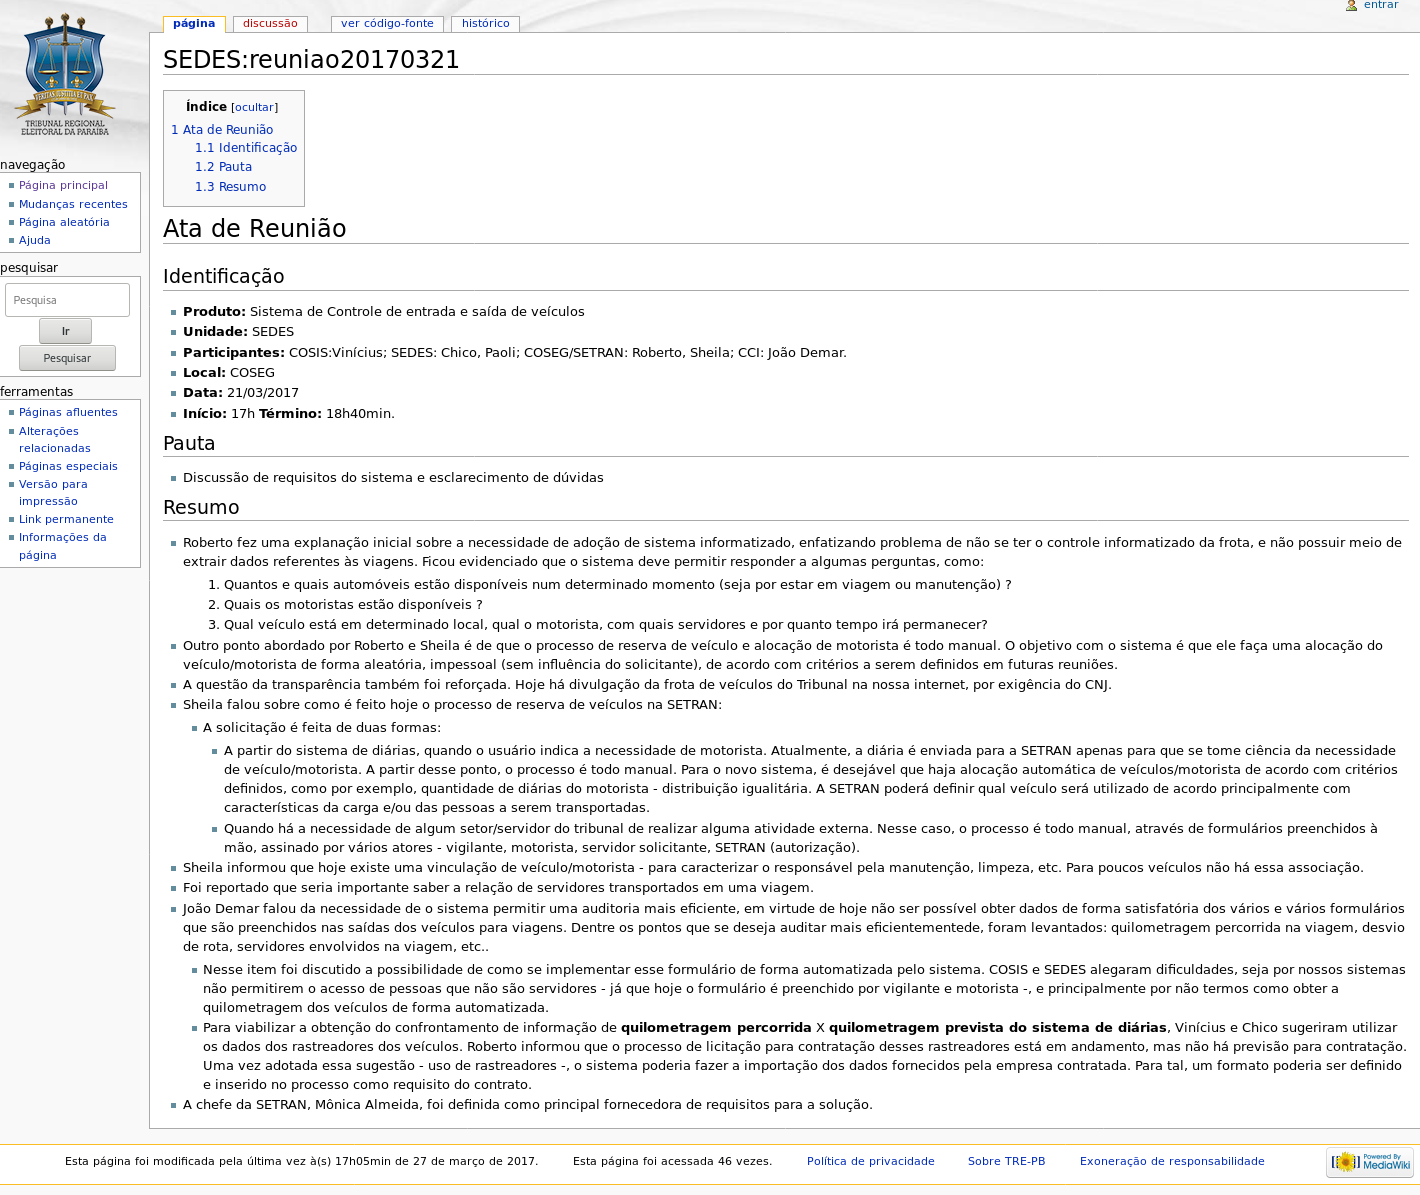
\includegraphics[width=0.9\textwidth]{dados/figuras/veiculos-reuniao20170321}
    \fonte{SEDES}
    \label{fig:figura-ataReuniao1}
\end{figure}

Posteriormente o time volta a se reunir e descrever as histórias de usuário na forma de requisitos a serem implementados. Com os requisitos descritos e cadastrados no sistema de gestão de projetos, o Redmine, na forma de tarefas e atividades, é possível mensurar o tamanho de cada atividade e assim estimar o tempo necessário para conclusão do projeto.  

\section{Planejamento}
\label{sec:atividadesRealizadasPlanejamento}

Todos os membros do time se reúnem para medir o tamanho de cada atividade. Uma a uma, as atividades são analisadas e discutidas por cada membro do time onde cada um expõe sua opinião e justifica o tamanho da atividade mesurado através da técnica do Planning Poker. Após um consenso entre todos, fica definido o tamanho da atividade. Assim o gerente com esses dados em mãos, formaliza o projeto como uma demanda de serviço, contendo o prazo e o time necessário para concluir as releases.

\begin{citacao}
Após a autorização, o gestor do sistema promoverá a reunião de
partida entre o time de desenvolvimento e as partes interessadas, momento em que será
esclarecido o problema de negócio, definidos papéis, explicado o processo de
desenvolvimento e distribuídas responsabilidades.\cite[p.~2]{Portaria37:2017}
\end{citacao}

As releases definidas são apresentadas como as versões que serão entregues e são separadas conforme ordem de prioridade das atividades e requisitos como mostra a \autoref{fig:figura-planejamento}.


\begin{figure}[!htb]
    \centering
    \caption{Planejamento das versões}
    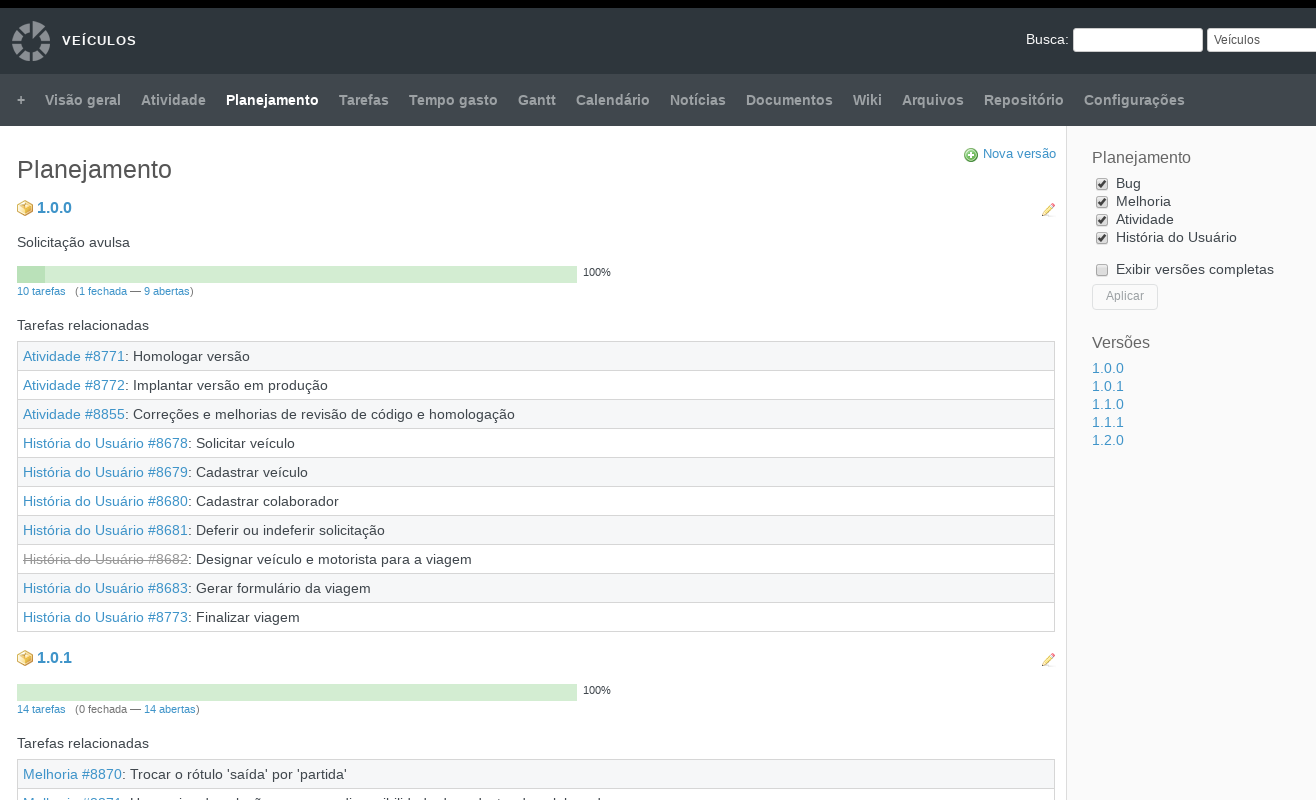
\includegraphics[width=0.75\textwidth]{dados/figuras/veiculos-planejamento.png}
    \fonte{SEDES}
    \label{fig:figura-planejamento}
\end{figure}

\section{Desenvolvimento}
\label{sec:atividadesRealizadasDesenvolvimento}

No início da fase de desenvolvimento são gerados os primeiros artefatos em código que serão comuns para todos os membros do time. O TRE-PB utiliza para controle de versões de seus códigos o sistema de versionamento denominado Subversion (SVN). Um novo repositório é criado para o projeto e um novo projeto com um arcabouço contendo as bibliotecas padrões e um template para as páginas já utilizadas pela SEDES é criado e disponibilizado no repositório para todos os desenvolvedores. A SISBAN. que através de um chamado, gera um novo schema no banco de dados Oracle 12g e fornece acesso a todos os desenvolvedores.

Todo esse processo é inicialmente implementado pelo supervisor técnico que geralmente é o desenvolvedor responsável pelo projeto e com mais habilidades e experiência do time.

Nesse momento todas as histórias já estão descritas com uma riqueza maior de detalhes, então são criados tickets e colados em um taskboard na forma de um quadro Kanban visível para todos. Esse quadro contém todas as atividades necessárias que atendem ao escopo do projeto para a release em questão. 

Diariamente são realizadas pequenas reuniões denominadas "daily" entre o gestor do projeto e membros do time com o intuito de detalhar o andamento das atividades, conduzir novas atividades para o time bem como relatar as dificuldades encontradas.

Na \autoref{fig:figura-atividade8940} a seguir é possível ver uma tarefa especifica que foi atribuída a mim. A tarefa cadastrada no Redmine possui uma ligação com o repositório SVN, assim é possível ver e analisar trechos de códigos que foram implementados em cada "commit"\footnote{No contexto de ciência da computação e gerenciamento de dados, commit refere-se à ideia de fazer permanentes um conjunto de mudanças experimentais. Uma utilização popular está no fim de uma transação. Um commit é o ato de enviar. https://pt.wikipedia.org/wiki/Commit}.

\begin{figure}[!htb]
    \centering
    \caption{Atividade 8940}
    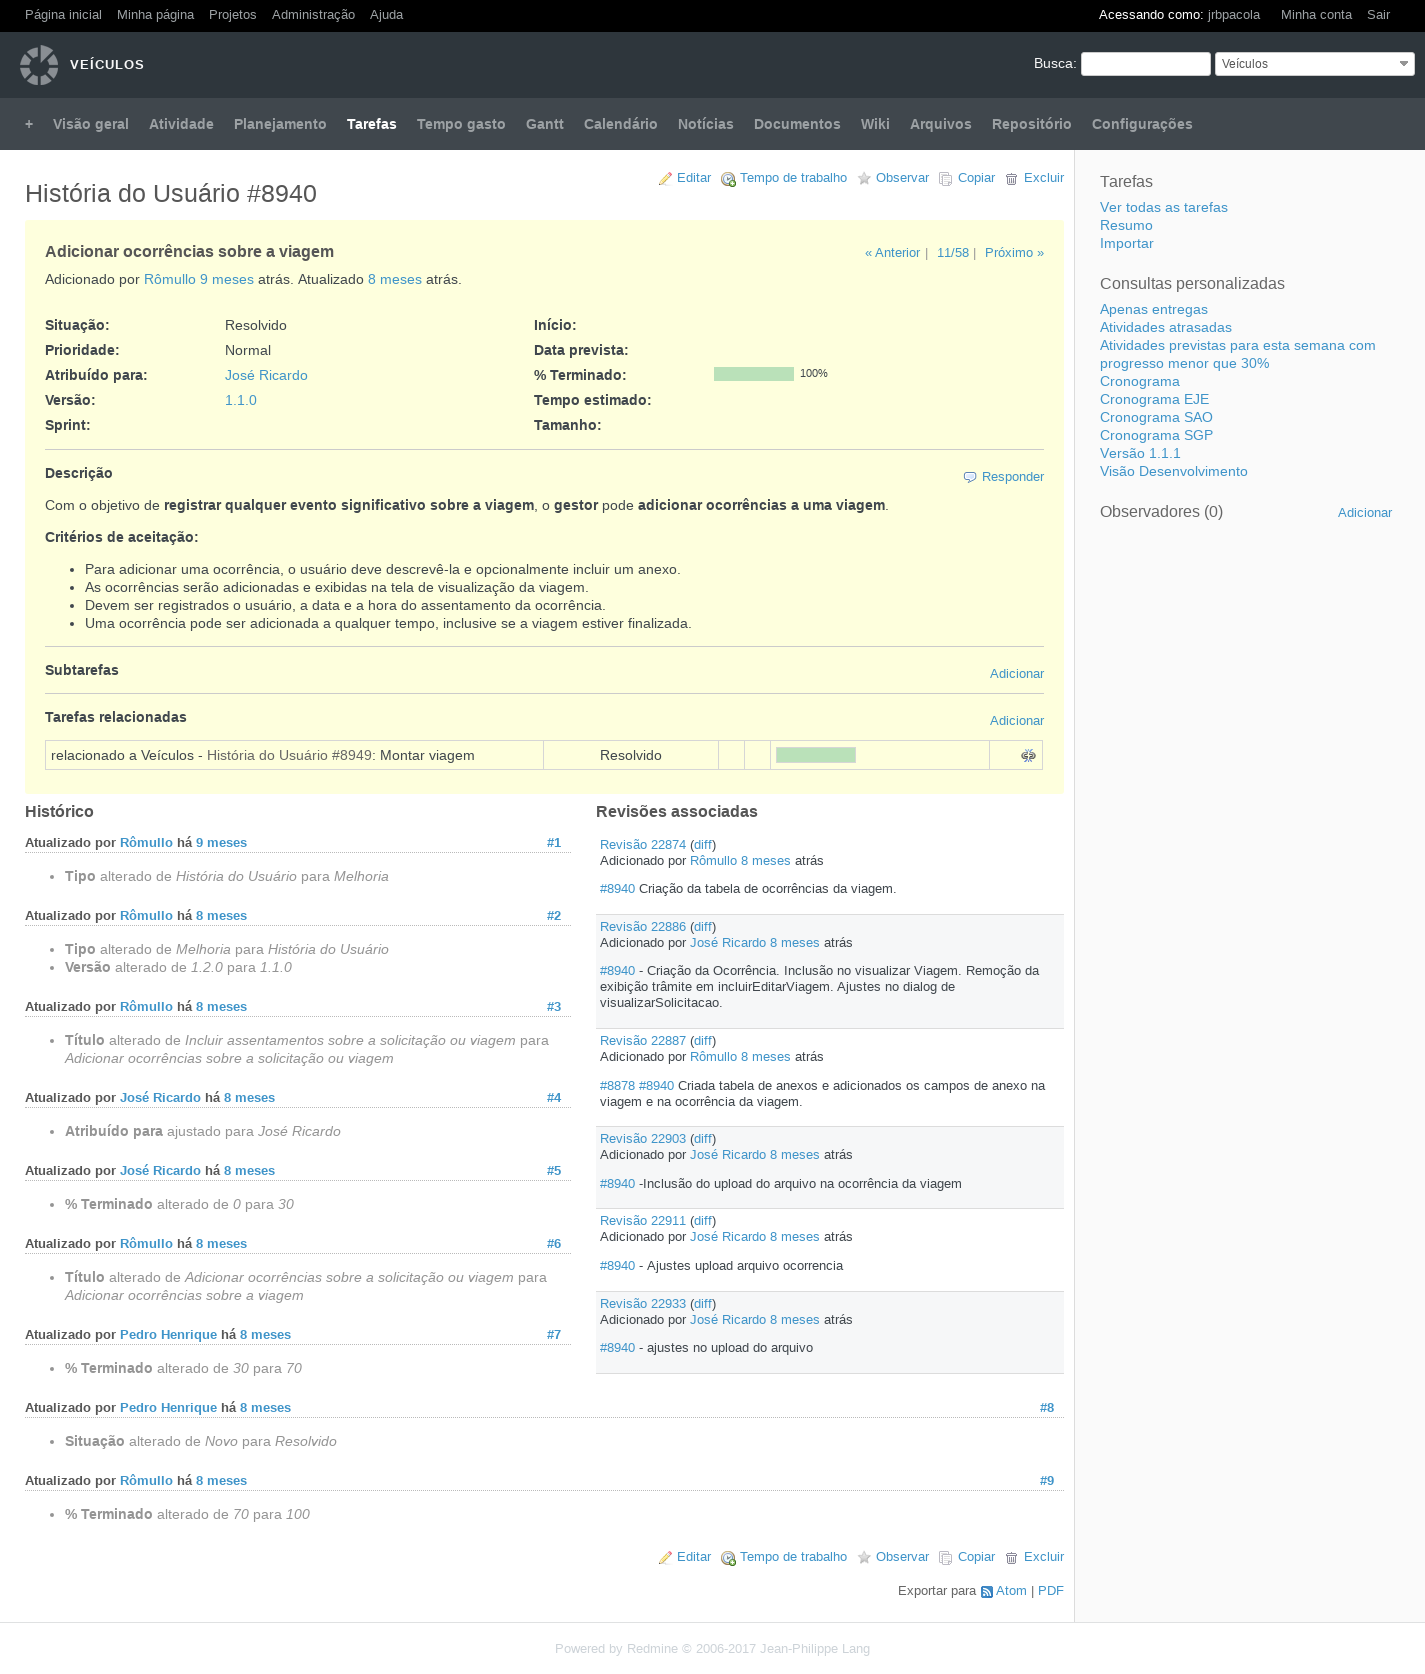
\includegraphics[width=0.75\textwidth]{dados/figuras/veiculos-atividade1.png}
    \fonte{SEDES}
    \label{fig:figura-atividade8940}
\end{figure}


\subsection{Criando as tabelas no banco}
\label{sbs:desenvolvimentoTabelas}

Com o domínio do problema já definido são então criadas as tabelas do banco de dados com seus atributos, relacionamentos e restrições.
Scripts em SQL são gerados, conforme exemplo da \autoref{fig:figura-scriptSQL}, para cada tabela, levando em consideração as particularidades da sintaxe SQL para o banco de dados Oracle. 

\begin{figure}[!htb]
    \centering
    \caption{Script SQL}
    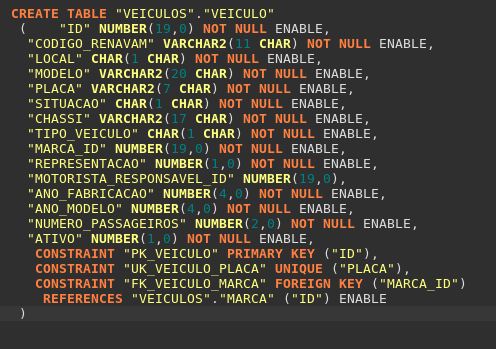
\includegraphics[width=0.75\textwidth]{dados/figuras/scriptSQL.png}
    \fonte{SEDES}
    \label{fig:figura-scriptSQL}
\end{figure}

\subsection{Mapeando o modelo com o banco}
\label{sbs:desenvolvimentoMapeamento}

Com as tabelas já criadas e relacionadas, começa-se a codificação propriamente dita na linguagem Java. As classes do modelo são codificadas com seus respectivos atributos e métodos e mapeadas através da interface JPA. Na \autoref{fig:figura-entidade} é possível ver a entidade que define um veículo na aplicação já com as anotações que a mapeiam com o banco de dados.

\begin{figure}[!htb]
    \centering
    \caption{Entidade Java - Veículo}
    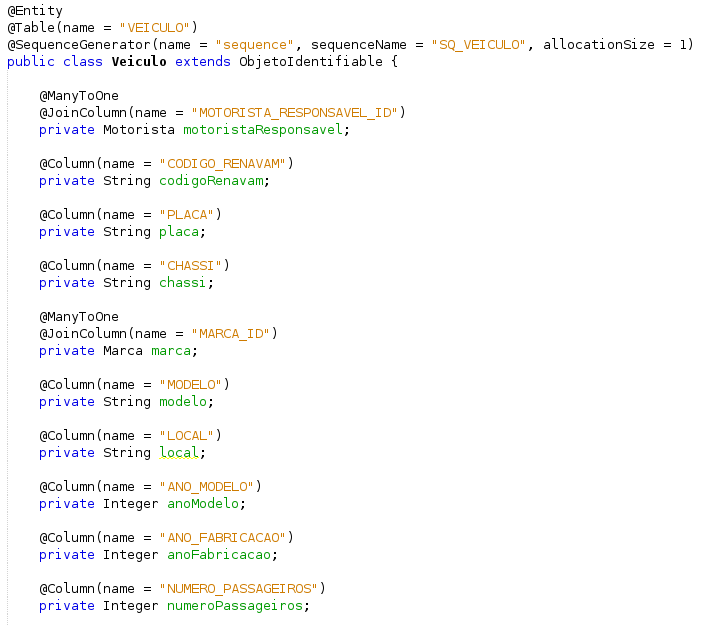
\includegraphics[width=0.75\textwidth]{dados/figuras/entidade.png}
    \fonte{SEDES}
    \label{fig:figura-entidade}
\end{figure}

      % Veículos
%% RESULTADOS-------------------------------------------------------------------

\chapter{ANÁLISE E DISCUSSÃO DOS RESULTADOS}

Cada capítulo deve conter uma pequena introdução (tipicamente, um ou dois parágrafos) que deve deixar claro o objetivo e o que será discutido no capítulo, bem como a organização do capítulo.
                    % Resultados
%% ORIENTAÇÕES GERAIS------------------------------------------------------------


% SOBRE AS ILUSTRAÇÕES----------------------------------------------------------
\chapter{SOBRE AS ILUSTRAÇÕES}
\label{chap:apSobreIlust}

A seguir exemplifica-se como inserir ilustrações no corpo do trabalho. As ilustrações serão indexadas automaticamente em suas respectivas listas. A numeração sequencial de figuras, tabelas e equações também ocorre de modo automático.

Referências cruzadas são obtidas através dos comandos \verb|\label{}| e \verb|\ref{}|. Sendo assim, não é necessário por exemplo, saber que o número de certo capítulo é \ref{chap:embasamentoTeorico} para colocar o seu número no texto. Outra forma que pode ser utilizada é esta: \autoref{chap:embasamentoTeorico}, facilitando a inserção, remoção e manejo de elementos numerados no texto sem a necessidade de renumerar todos esses elementos.

% FIGURAS-----------------------------------------------------------------------
\chapter{FIGURAS}
\label{chap:figuras}

Exemplo de como inserir uma figura. A \autoref{fig:figura-exemplo1} aparece automaticamente na lista de figuras. Para saber mais sobre o uso de imagens no \LaTeX{} consulte literatura especializada \cite{Goossens2007}.

Os arquivos das figuras devem ser armazenados no diretório de "/dados".

\begin{figure}[!htb]
    \centering
    \caption{Exemplo de Figura}
    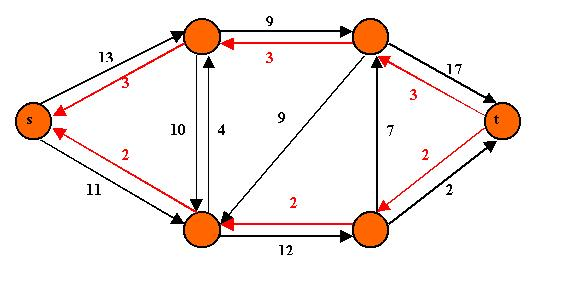
\includegraphics[width=0.5\textwidth]{./dados/figuras/figura1}
    \fonte{\citeonline{IRL2014}}
    \label{fig:figura-exemplo1}
\end{figure}

% QUADROS E TABELAS---------------------------------------------------------------
\chapter{QUADROS E TABELAS}
\label{chap:tabelas}

Exemplo de como inserir o \autoref{qua:quadro-exemplo1} e a \autoref{tab:tabela-exemplo1}. Ambos aparecem automaticamente nas suas respectivas listas. Para saber mais informações sobre a construção de tabelas no \LaTeX{} consulte literatura especializada \cite{Mittelbach2004}.

Ambos os elementos (Quadros e Tabelas) devem ser criados em arquivos separados para facilitar manutenção e armazenados no diretório de "/dados".

\begin{quadro}[!htb]
    \centering
    \caption{Exemplo de Quadro.\label{qua:quadro-exemplo1}}
    \begin{tabular}{|p{7cm}|p{7cm}|}
        \hline
        \textbf{BD Relacionais} & \textbf{BD Orientados a Objetos} \\
        \hline
        Os dados são passivos, ou seja, certas operações limitadas podem ser automaticamente acionadas quando os dados são usados. Os dados são ativos, ou seja, as solicitações fazem com que os objetos executem seus métodos. & Os processos que usam dados mudam constantemente. \\
        \hline
    \end{tabular}
    \fonte{\citeonline{Barbosa2004}}
\end{quadro}


A diferença entre quadro e tabela está no fato que um quadro é formado por linhas horizontais e verticais. Deve ser utilizado quando o conteúdo é majoritariamente não-numérico. O número do quadro e o título vem acima do quadro, e a fonte, deve vir abaixo. E Uma tabela é formada apenas por linhas verticais. Deve ser utilizada quando o conteúdo é majoritariamente numérico. O número da tabela e o título vem acima da tabela, e a fonte, deve vir abaixo, tal como no quadro.

\begin{table}[!htb]
    \centering
    \caption[Resultado dos testes]{Resultado dos testes.
    \label{tab:tabela-exemplo1}}
    \begin{tabular}{rrrrr}
        \toprule
            & Valores 1 & Valores 2 & Valores 3 & Valores 4 \\
        \midrule
            Caso 1 & 0,86 & 0,77 & 0,81 & 163 \\
            Caso 2 & 0,19 & 0,74 & 0,25 & 180 \\
            Caso 3 & 1,00 & 1,00 & 1,00 & 170 \\
        \bottomrule
    \end{tabular}
    \fonte{\citeonline{Barbosa2004}}
\end{table}


% EQUAÇÕES-----------------------------------------------------------------------
\chapter{EQUAÇÕES}
\label{chap:equacoes}

Exemplo de como inserir a \autoref{eq:equacao-exemplo1} e a Eq. \ref{eq:equacao-exemplo2} no corpo do texto \footnote{Deve-se atentar ao fato de a formatação das equações ficar muito boa esteticamente.}. Observe que foram utilizadas duas formas distintas para referenciar as equações.

\begin{equation}
    X(s) = \int\limits_{t = -\infty}^{\infty} x(t) \, \text{e}^{-st} \, dt
    \label{eq:equacao-exemplo1}
\end{equation}

\begin{equation}
    F(u, v) = \sum_{m = 0}^{M - 1} \sum_{n = 0}^{N - 1} f(m, n) \exp \left[ -j 2 \pi \left( \frac{u m}{M} + \frac{v n}{N} \right) \right]
    \label{eq:equacao-exemplo2}
\end{equation}

% ALGORITMOS-----------------------------------------------------------------------
\chapter{ALGORITMOS}
\label{chap:algoritmos}

Exemplo de como inserir um algoritmo. Para inserção de algoritmos utiliza-se o pacote {\ttfamily algorithm2e} que já está devidamente configurado dentro do template.

Os algoritmos devem ser criados em arquivos separados para facilitar manutenção e armazenados no diretório de "/dados".\\
\\

\begin{algorithm}
    \caption{Exemplo de Algoritmo}
    \KwIn{o número $n$ de vértices a remover, grafo original $G(V, E)$}
    \KwOut{grafo reduzido $G'(V,E)$}
    $removidos \leftarrow 0$ \\
    \While {removidos $<$ n } {
        $v \leftarrow$ Random$(1, ..., k) \in V$ \\
            \For {$u \in adjacentes(v)$} {
                remove aresta (u, v)\\
                $removidos \leftarrow removidos + 1$\\
            }
            \If {há  componentes desconectados} {
                remove os componentes desconectados\\
            }
        }
\end{algorithm}


% SOBRE AS LISTAS--------------------------------------------------------------------
\chapter{SOBRE AS LISTAS}
\label{chap:apSobreLista}

Para construir listas de "\textit{bullets}"{} ou listas enumeradas, inclusive listas aninhadas, é utilizado o pacote \verb|paralist|.

Exemplo de duas listas não numeradas aninhadas, utilizando o comando \verb|\itemize|. Observe a indentação, bem como a mudança automática do tipo de "\textit{bullet}"{} nas listas aninhadas.

\begin{itemize}
    \item item não numerado 1
    \item item não numerado 2
    \begin{itemize}
        \item subitem não numerado 1
        \item subitem não numerado 2
        \item subitem não numerado 3
    \end{itemize}
    \item item não numerado 3
\end{itemize}

Exemplo de duas listas numeradas aninhadas, utilizando o comando \verb|\enumerate|. Observe a numeração progressiva e indentação das listas aninhadas.

\begin{enumerate}
    \item item numerado 1
    \item item numerado 2
    \begin{enumerate}
        \item subitem numerado 1
        \item subitem numerado 2
        \item subitem numerado 3
    \end{enumerate}
    \item item numerado 3
\end{enumerate}

% SOBRE AS CITAÇÕES E CHAMADAS DE REFERÊNCAS----------------------------------------------
\chapter{SOBRE AS CITAÇÕES E CHAMADAS DE REFERÊNCAS}
\label{chap:apSobreCita}

Citações são trechos de texto ou informações obtidas de materiais consultadss quando da elaboração do trabalho. São utilizadas no texto com o propósito de esclarecer, completar e embasar as ideias do autor. Todas as publicações consultadas e utilizadas (por meio de citações) devem ser listadas, obrigatoriamente, nas referências bibliográficas, para preservar os direitos autorais. São classificadas em citações indiretas e diretas.

% CITAÇÕES INDIRETAS-----------------------------------------------------------------------
\chapter{CITAÇÕES INDIRETAS}
\label{chap:citacoesLivres}

É a transcrição, com suas próprias palavras, das idéias de um autor, mantendo-se o sentido original. A citação indireta é a maneira que o pesquisador tem de ler, compreender e gerar conhecimento a partir do conhecimento de outros autores. Quanto à chamada da referência, ela pode ser feita de duas maneiras distintas, conforme o nome do(s) autor(es) façam parte do seu texto ou não. Exemplo de chamada fazendo parte do texto:\\
\\Enquanto \citeonline{Maturana2003} defendem uma epistemologia baseada na biologia. Para os autores, é necessário rever \ldots.\\

A chamada de referência foi feita com o comando \verb|\citeonline{chave}|, que produzirá a formatação correta.

A segunda forma de fazer uma chamada de referência deve ser utilizada quando se quer evitar uma interrupção na sequência do texto, o que poderia, eventualmente, prejudicar a leitura. Assim, a citação é feita e imediatamente após a obra referenciada deve ser colocada entre parênteses. Porém, neste caso específico, o nome do autor deve vir em caixa alta, seguido do ano da publicação. Exemplo de chamada não fazendo parte do texto:\\
\\Há defensores da epistemologia baseada na biologia que argumentam em favor da necessidade de \ldots \cite{Maturana2003}.\\

Nesse caso a chamada de referência deve ser feita com o comando \verb|\cite{chave}|, que produzirá a formatação correta.

% CITAÇÕES DIRETAS-----------------------------------------------------------------------
\chapter{CITAÇÕES DIRETAS}
\label{chap:citacoesLiterais}

É a transcrição ou cópia de um parágrafo, de uma frase, de parte dela ou de uma expressão, usando exatamente as mesmas palavras adotadas pelo autor do trabalho consultado.

Quanto à chamada da referência, ela pode ser feita de qualquer das duas maneiras já mencionadas nas citações indiretas, conforme o nome do(s) autor(es) façam parte do texto ou não. Há duas maneiras distintas de se fazer uma citação direta, conforme o trecho citado seja longo ou curto.

Quando o trecho citado é longo (4 ou mais linhas) deve-se usar um parágrafo específico para a citação, na forma de um texto recuado (4 cm da margem esquerda), com tamanho de letra menor e espaçamento entrelinhas simples. Exemplo de citação longa:
\\\begin{citacao}
    Desse modo, opera-se uma ruptura decisiva entre a reflexividade filosófica, isto é a possibilidade do sujeito de pensar e de refletir, e a objetividade científica. Encontramo-nos num ponto em que o conhecimento científico está sem consciência. Sem consciência moral, sem consciência reflexiva e também subjetiva. Cada vez mais o desenvolvimento extraordinário do conhecimento científico vai tornar menos praticável a própria possibilidade de reflexão do sujeito sobre a sua pesquisa \cite[p.~28]{Silva2000}.
\end{citacao}

Para fazer a citação longa deve-se utilizar os seguintes comandos:
\begin{verbatim}
\begin{citacao}
<texto da citacao>
\end{citacao}
\end{verbatim}

No exemplo acima, para a chamada da referência o comando \verb|\cite[p.~28]{Silva2000}| foi utilizado, visto que os nomes dos autores não são parte do trecho citado. É necessário também indicar o número da página da obra citada que contém o trecho citado.

Quando o trecho citado é curto (3 ou menos linhas) ele deve inserido diretamente no texto entre aspas. Exemplos de citação curta:\\
\\A epistemologia baseada na biologia parte do princípio de que "assumo que não posso fazer referência a entidades independentes de mim para construir meu explicar" \cite[p.~35]{Maturana2003}.\\
\\A epistemologia baseada na biologia de \citeonline[p.~35]{Maturana2003} parte do princípio de que "assumo que não posso fazer referência a entidades independentes de mim para construir meu explicar".

% DETALHES SOBRE AS CHAMADAS DE REFERÊNCIAS---------------------------------------------------------
\chapter{DETALHES SOBRE AS CHAMADAS DE REFERÊNCIAS}
\label{chap:referUtilizadas}

Outros exemplos de comandos para as chamadas de referências e o resultado produzido por estes:\\
\\\citeonline{Maturana2003} \ \ \  \verb|\citeonline{Maturana2003}|\\
\citeonline{Barbosa2004} \ \ \   \verb|\citeonline{Barbosa2004}|\\
\cite[p.~28]{Silva2000} \ \ \  \verb|\cite[p.~28]{Silva2000}|\\
\citeonline[p.~33]{Silva2000} \ \ \   \verb|\citeonline[p.~33]{v}|\\
\cite[p.~35]{Maturana2003} \ \ \   \verb|\cite[p.~35]{Maturana2003}|\\
\citeonline[p.~35]{Maturana2003} \ \ \   \verb|\citeonline[p.~35]{Maturana2003}|\\
\cite{Barbosa2004,Maturana2003} \ \ \   \verb|\cite{Barbosa2004,Maturana2003}|\\

% SOBRE AS REFERÊNCIAS BIBLIOGRÁFICAS-------------------------------------------------------
\chapter{SOBRE AS REFERÊNCIAS BIBLIOGRÁFICAS}
\label{chap:apSobreRefer}

A bibliografia é feita no padrão \textsc{Bib}\TeX{}. As referências são colocadas em um arquivo separado. Neste template as referências são armazenadas no arquivo "base-referencias.bib".

Existem diversas categorias documentos e materiais componentes da bibliografia. A classe abn\TeX{} define as seguintes categorias (entradas):

\begin{verbatim}
@book
@inbook
@article
@phdthesis
@mastersthesis
@monography
@techreport
@manual
@proceedings
@inproceedings
@journalpart
@booklet
@patent
@unpublished
@misc
\end{verbatim}

Cada categoria (entrada) é formatada pelo pacote \citeonline{abnTeX22014d} de uma forma específica. Algumas entradas foram introduzidas especificamente para atender à norma \citeonline{NBR6023:2002}, são elas: \verb|@monography|, \verb|@journalpart|,\verb|@patent|. As demais entradas são padrão \textsc{Bib}\TeX{}. Para maiores detalhes, refira-se a \citeonline{abnTeX22014d}, \citeonline{abnTeX22014b}, \citeonline{abnTeX22014c}.

% NOTAS DE RODAPÉ--------------------------------------------------------------------------
\chapter{NOTAS DE RODAPÉ}
\label{chap:notasRodape}

As notas de rodapé pode ser classificadas em duas categorias: notas explicativas\footnote{é o tipo mais comum de notas que destacam, explicam e/ou complementam o que foi dito no corpo do texto, como esta nota de rodapé, por exemplo.} e notas de referências. A notas de referências, como o próprio nome ja indica, são utilizadas para colocar referências e/ou chamadas de referências sob certas condições.

                   % Capítulo com Orientações de uso do Template
% CONSIDERAÇÕES FINAIS--------------------------------------------------------------------

\chapter{Considerações Finais}
\label{chap:consideracoesFinais}

% TODO: ajustar a conclusão, incluir futuras versões, relatar mais claramente sua função e o qual foi a importância para o projeto.

O sistema passou a ser utilizado em sua plenitude a partir de agosto de 2017 e em 2018 terminou o ano sendo o 4º sistema mais usado em todo o TRE com 23.375 transações conforme \autoref{fig:figura-ranking2018}. Já em 2019, até março foram registradas 4.006 transações já sendo o 3º sistema mais utilizado como pode ser visto na \autoref{fig:figura-ranking2019}.

\begin{figure}[!htb]
    \centering
    \caption{Veículos - Ranking 2018}
    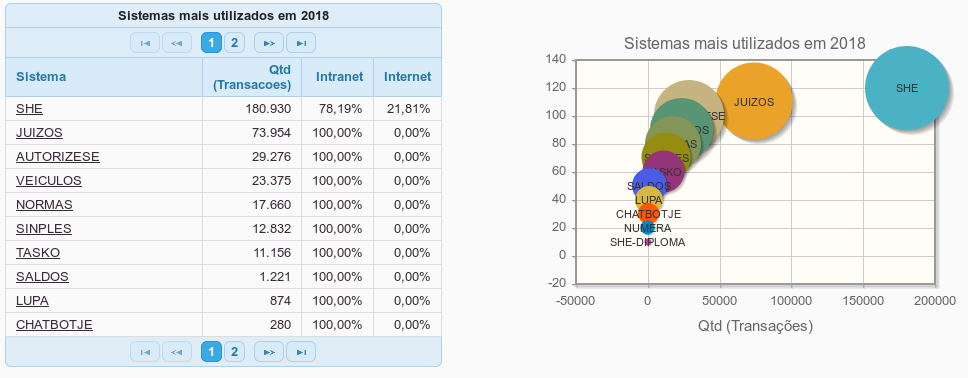
\includegraphics[width=0.75\textwidth]{./dados/figuras/ranking2018.png}
    \fonte{SEDES}
    \label{fig:figura-ranking2018}
\end{figure}

\begin{figure}[!htb]
    \centering
    \caption{Veículos - Ranking 2019}
    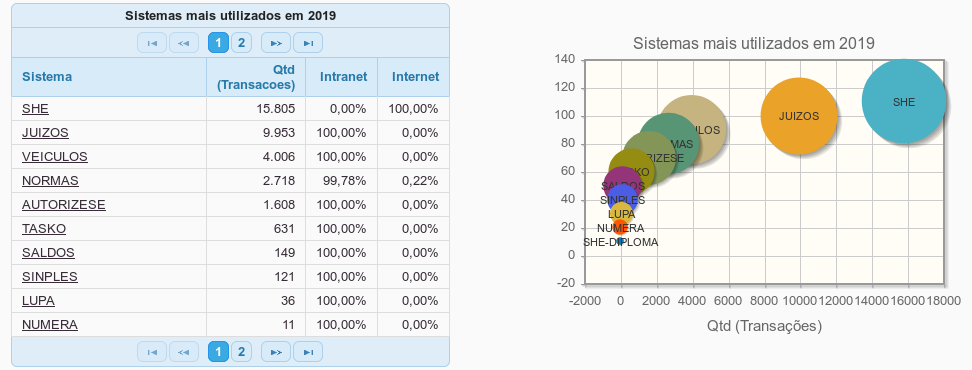
\includegraphics[width=0.75\textwidth]{./dados/figuras/ranking2019.png}
    \fonte{SEDES}
    \label{fig:figura-ranking2019}
\end{figure}

A experiência de estágio no TRE-PB adicionou propriedade aos conhecimentos adquiridos ao longo da minha jornada como aluno e desenvolvedor de sistemas para internet. 
Durante os dois anos de estágio fui incluído em uma rotina de trabalho equivalente as teorias e práticas vistas e desenvolvidas em sala de aula. 
Fui amparado por excelentes profissionais, sempre dispostos a dar o seu melhor tanto para o ambiente de trabalho quanto para uma sociedade melhor e mais justa.

Assistir uma boa aula, realizar os exercícios em sala e ainda repetir todo esse processo durante o estágio proporcionou, sem dúvidas, um crescimento imensurável ao meu intelecto. Tive a oportunidade de participar de alguns projetos, dentre eles o \imprimirtitulo \space, o qual participei já na primeira reunião até seu encerramento. Poder opinar, dar sugestões, incluir classes inteiras ao projeto, compilar o código e realizar o deploy da aplicação, até mesmo em produção me fez acreditar que eu estava no caminho correto e que seria possível me apresentar diante de qualquer empresa como um verdadeiro profissional.

Durante o projeto me deparei com situações de grande dificuldade, as vezes por não conseguir codificar a solução do problema, outras pelo tamanho da responsabilidade envolvida. Sempre fui encorajado a encontrar a solução, investigar, às vezes por dias.
Fiz parte de uma equipe sempre pronta e disposta a resolver suas demandas de trabalho, esclarecer dúvidas, sempre discutindo possibilidades de melhorar. Sinto orgulho em dizer que, durante meu estágio, todos os desenvolvedores efetivos do TRE-PB foram alunos IFPB.

Saio satisfeito dessa jornada, sabendo que pude absorver o máximo do que foi exposto durante o curso e o estágio. Tratando-se de tecnologias, muito ainda é pouco. Tudo que aprendi e vivi serve apenas como base para minha carreira como desenvolvedor. Conquistei apenas a ponta do iceberg, tenho plena clareza que falta muito a aprender e evoluir ainda.                  			   % Conclusão

\postextual
% INSERE ELEMENTOS PÓS-TEXTUAIS
% REFERÊNCIAS------------------------------------------------------------------

% Carrega o arquivo "base-referencias.bib" e extrai automaticamente as referências citadas

\bibliography{./base-referencias}
\bibliographystyle{abntex2-alf} % Define o estilo ABNT para formatar a lista de referências
% OBSERVAÇÕES------------------------------------------------------------------
% Este arquivo não precisa ser alterado.
           			   % Referências
% APÊNDICES--------------------------------------------------------------------

\begin{apendicesenv}
\partapendices

% Primeiro apêndice------------------------------------------------------------
\chapter{Nome do apêndice} % Edite para alterar o título deste apêndice
\label{chap:apendiceA}

Lembre-se que a diferença entre apêndice e anexo diz respeito à autoria do texto e/ou material ali colocado.

Caso o material ou texto suplementar ou complementar seja de sua autoria, então ele deverá ser colocado como um apêndice. Porém, caso a autoria seja de terceiros, então o material ou texto deverá ser colocado como anexo.

Caso seja conveniente, podem ser criados outros apêndices para o seu trabalho acadêmico. Basta recortar e colar este trecho neste mesmo documento. Lembre-se de alterar o "label"{} do apêndice.

Não é aconselhável colocar tudo que é complementar em um único apêndice. Organize os apêndices de modo que, em cada um deles, haja um único tipo de conteúdo. Isso facilita a leitura e compreensão para o leitor do trabalho.

% Novo apêndice----------------------------------------------------------------
\chapter{Nome do outro apêndice}
\label{chap:apendiceB}

conteúdo do novo apêndice

\end{apendicesenv}
             			   % Apêndices
% ANEXO------------------------------------------------------------------------

\begin{anexosenv}
\partanexos

% Primeiro anexo---------------------------------------------------------------
\chapter{Modus 3.1}     % edite para alterar o título deste anexo
\label{chap:anexoA}
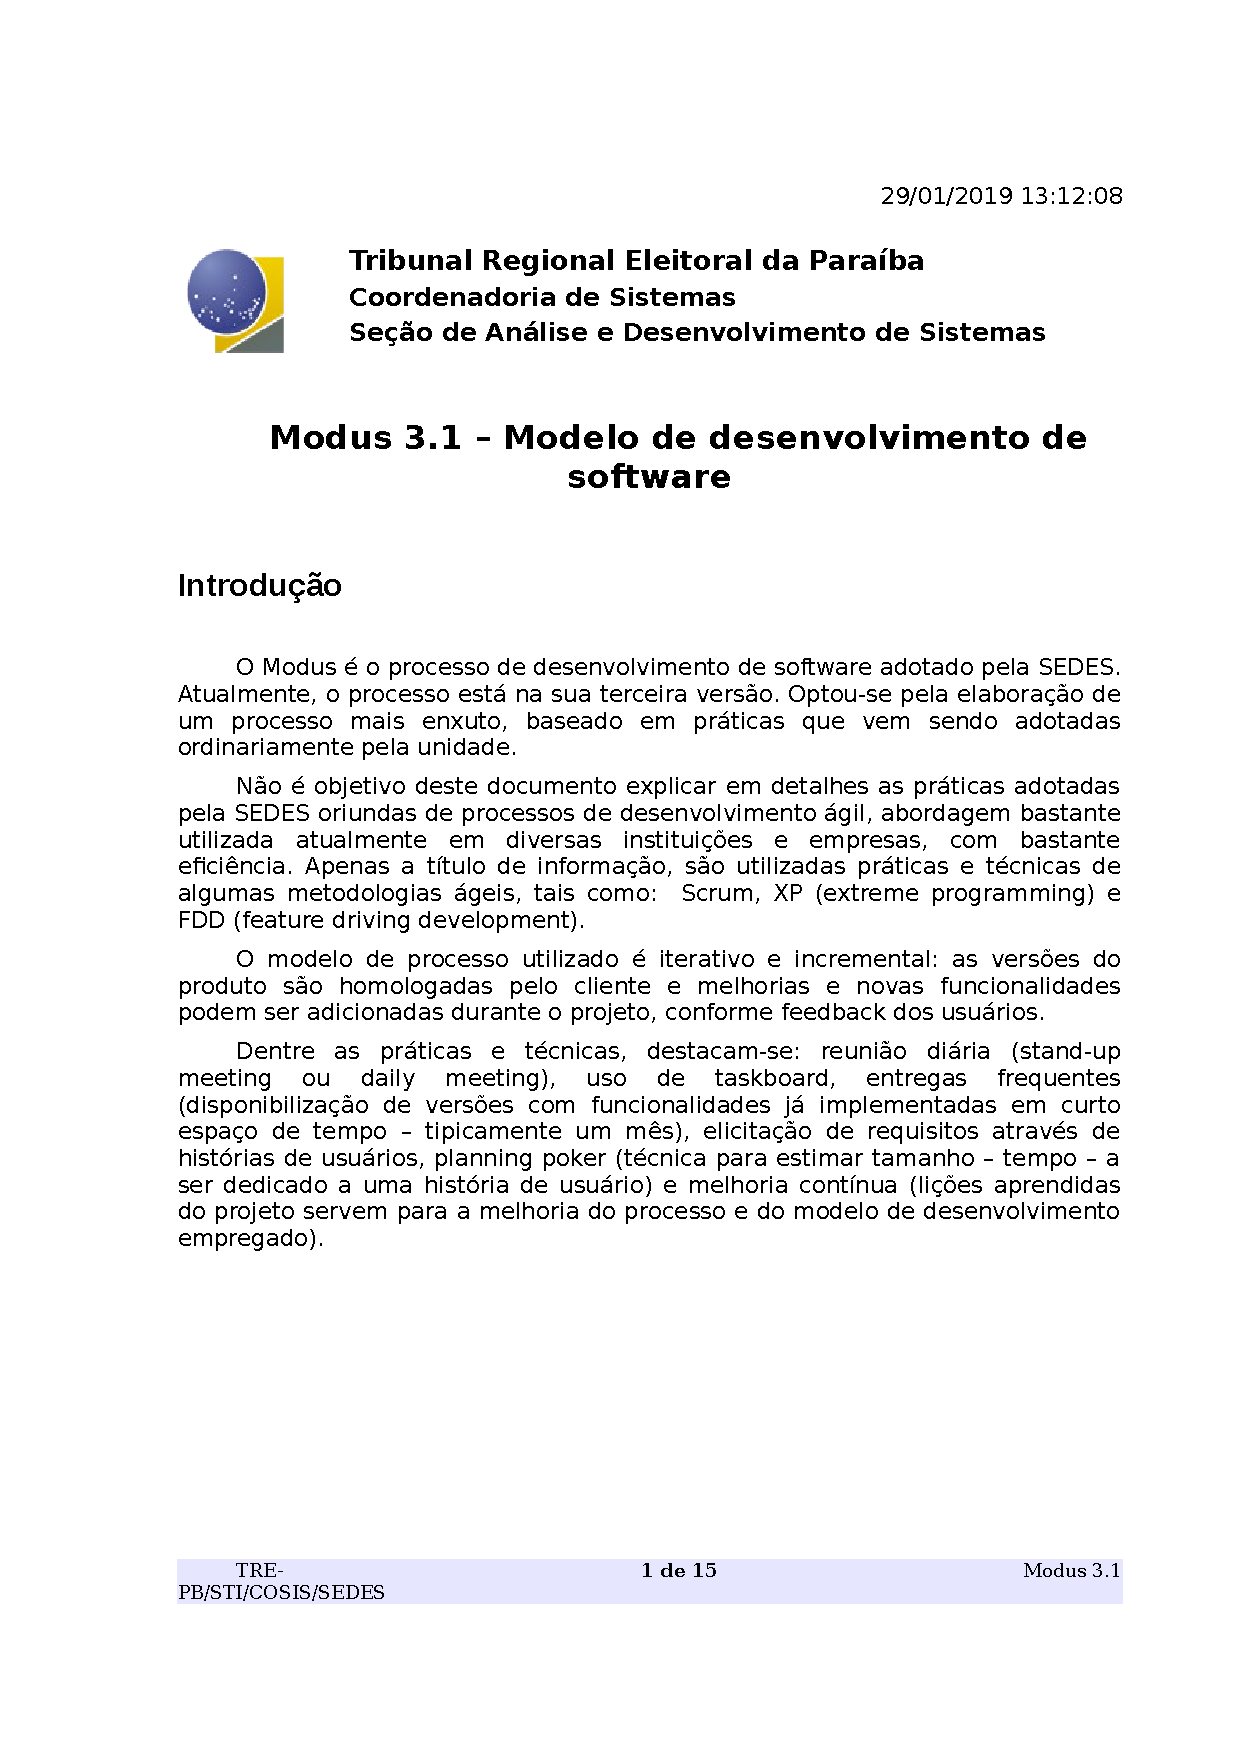
\includepdf[pages=-]{./dados/anexos/Modus_3_1.pdf}


% Novo anexo-------------------------------------------------------------------
\chapter{Portaria 37/2017}
\label{chap:anexoB}
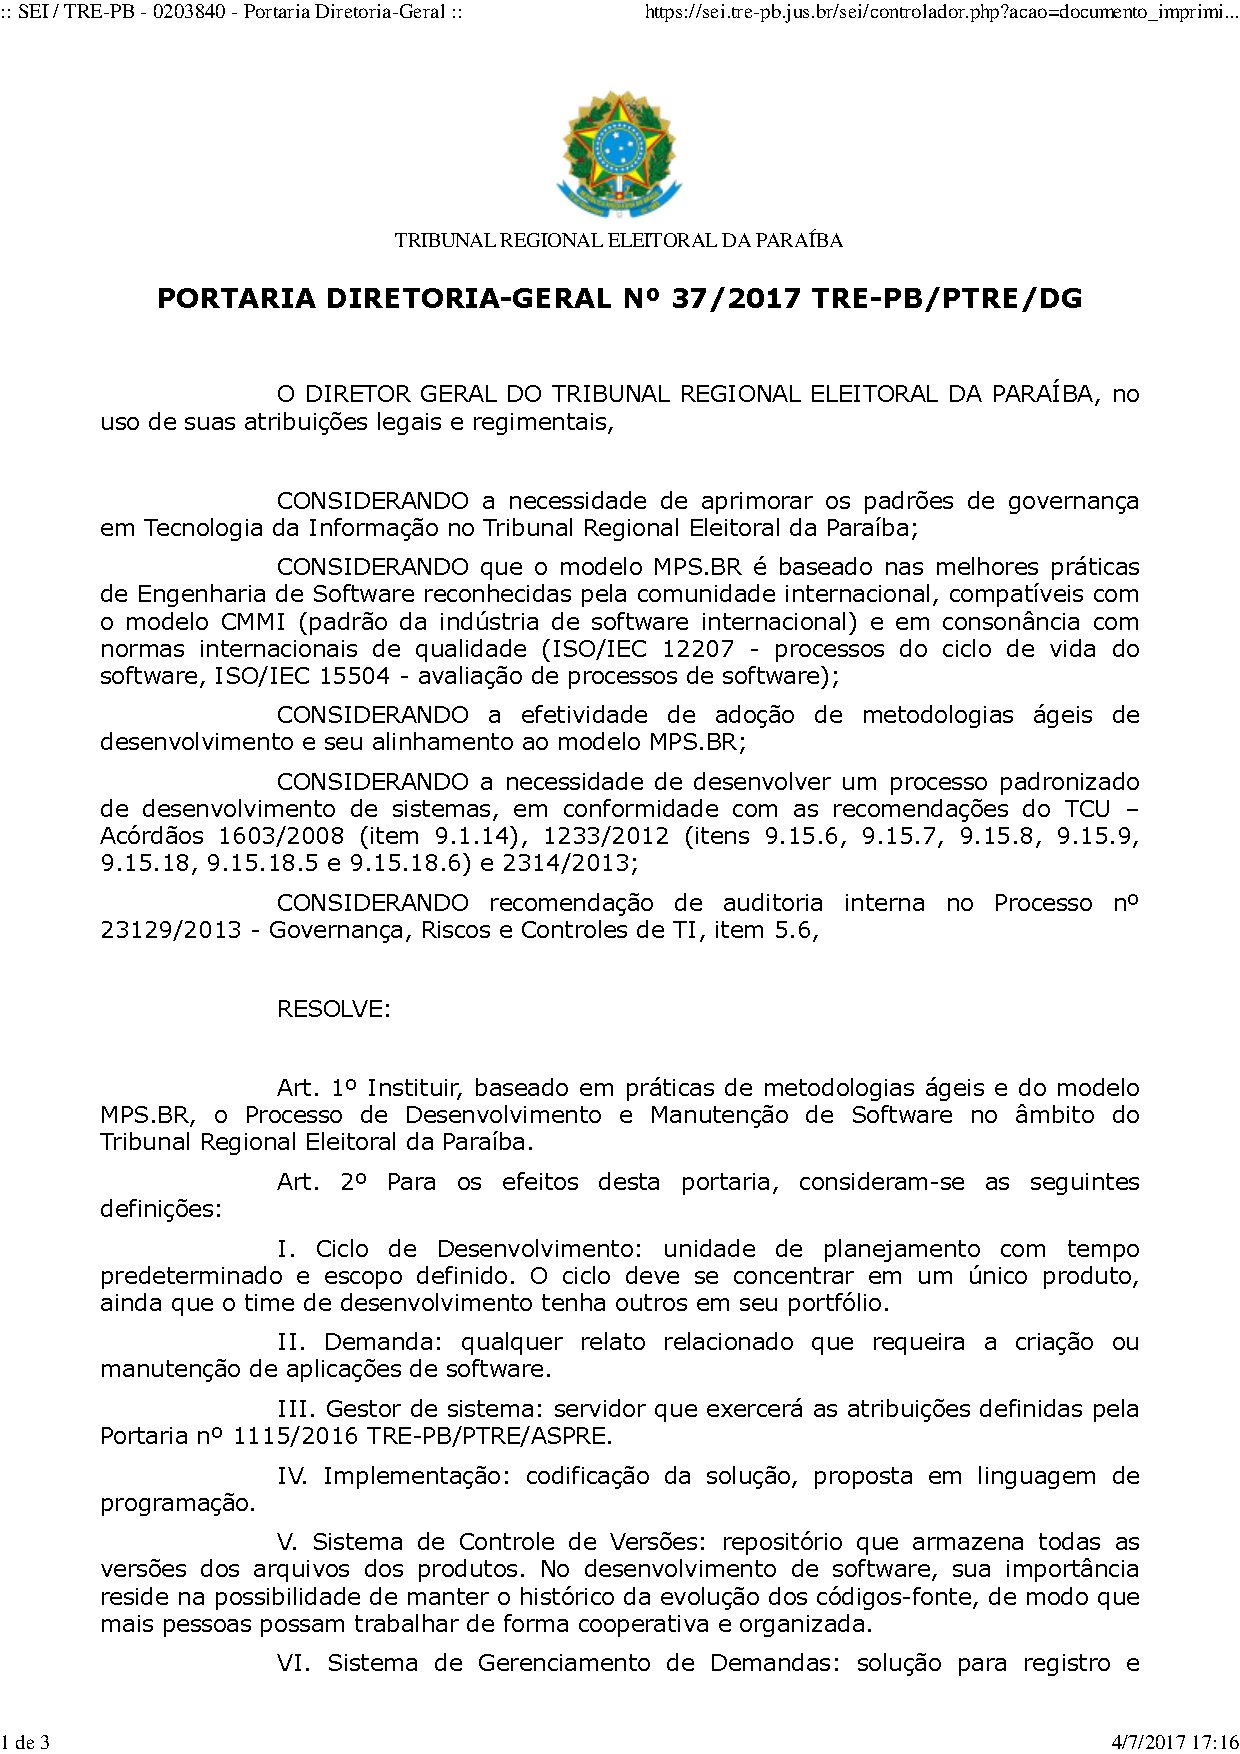
\includepdf[pages=-]{./dados/anexos/TRE-PB-portaria-37-2017.pdf}

\end{anexosenv}
               			   % Anexos

\end{document}
